\documentclass[../thesis.tex]{subfiles}
\begin{document}
\graphicspath{ {./img/}{./tab/} }
\section[]{High-order implicit schemes in 1D}
We are interested in constructing implicit finite volume schemes that can be solved efficiently. Thus, e.g., yields a similar system of equations as in the case of implicit-upwind scheme.
As a guidance, let us use our knowledge of the solutions of the advection equation. In that case we know that the solution at a later time is the translated initial condition, see Figure~\ref{fig:characteristics-1d}.
\begin{figure}[H]
	\centering
	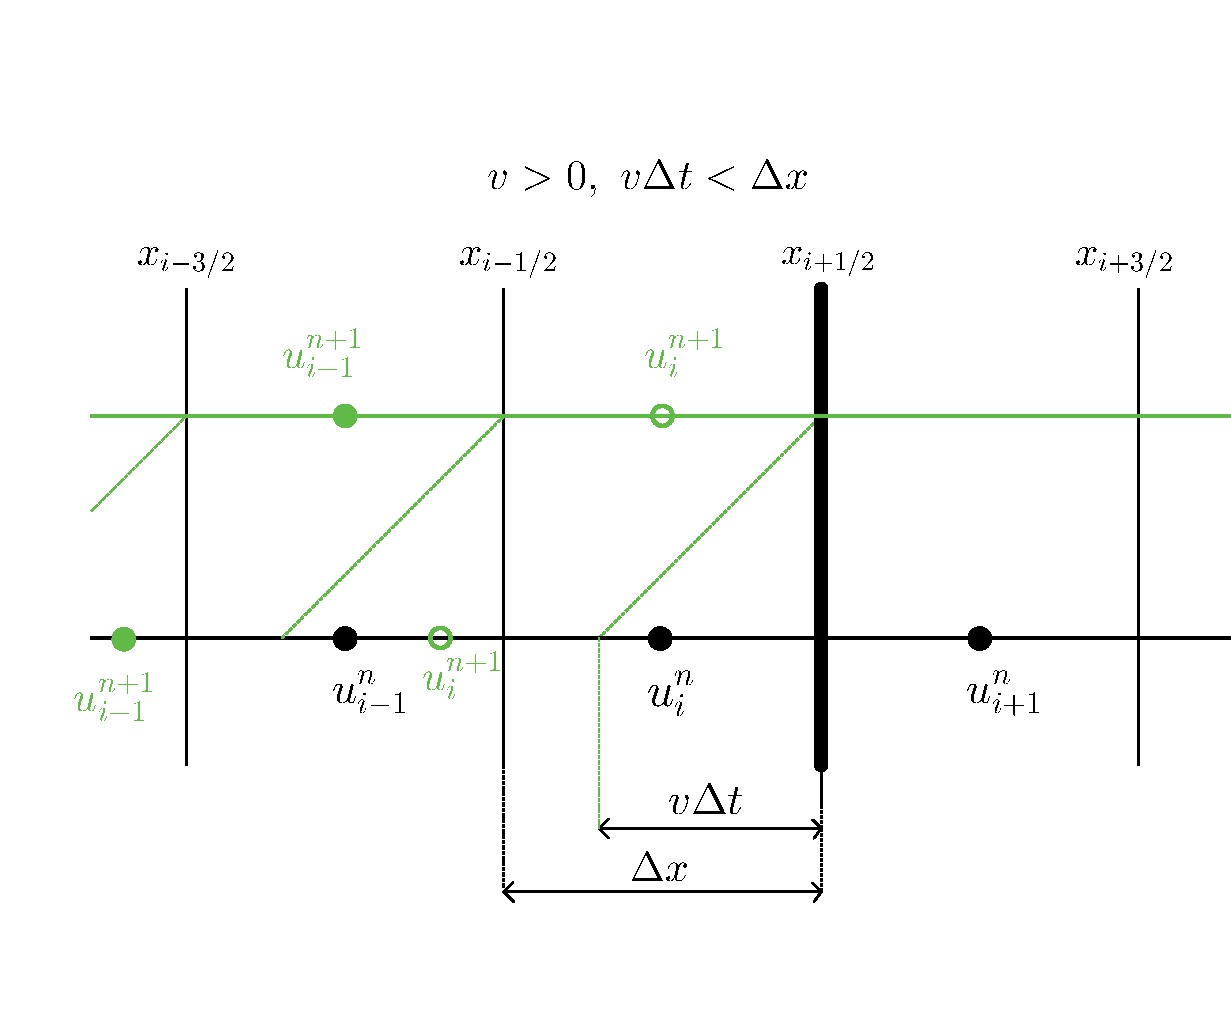
\includegraphics[width=\textwidth]{Characteristics-crop.pdf}
	\caption{Averages in \(x-t\) coordinates}
	\label{fig:characteristics-1d}
\end{figure}
A particular finite volume scheme is defined by the definition of the numerical flux through the cell interface, thus, how it approximates the flow of a quantity through a surface in a given time interval.
Our goal is to compute the flux through the face at \(x_{i+1/2}\) using the known cell averages.
For convenience, we shift to space coordinates.
This way we can see the connection directly between well established explicit schemes based on polynomial reconstruction \cite{1977_VanLeer,2002_LeVeque_BOOK} and our implicit schemes.
We could equivalently shift to time coordinates, as it was done in, e.g., \cite{2023_Barsukow,2022_Eimer}.
We are interested in compact schemes in a sense that to compute the time-average of the flux through the face at \(x_{i+1/2}\) we want to use the stencil \(i-1, i, i+1\).
\begin{figure}[H]
	\centering
	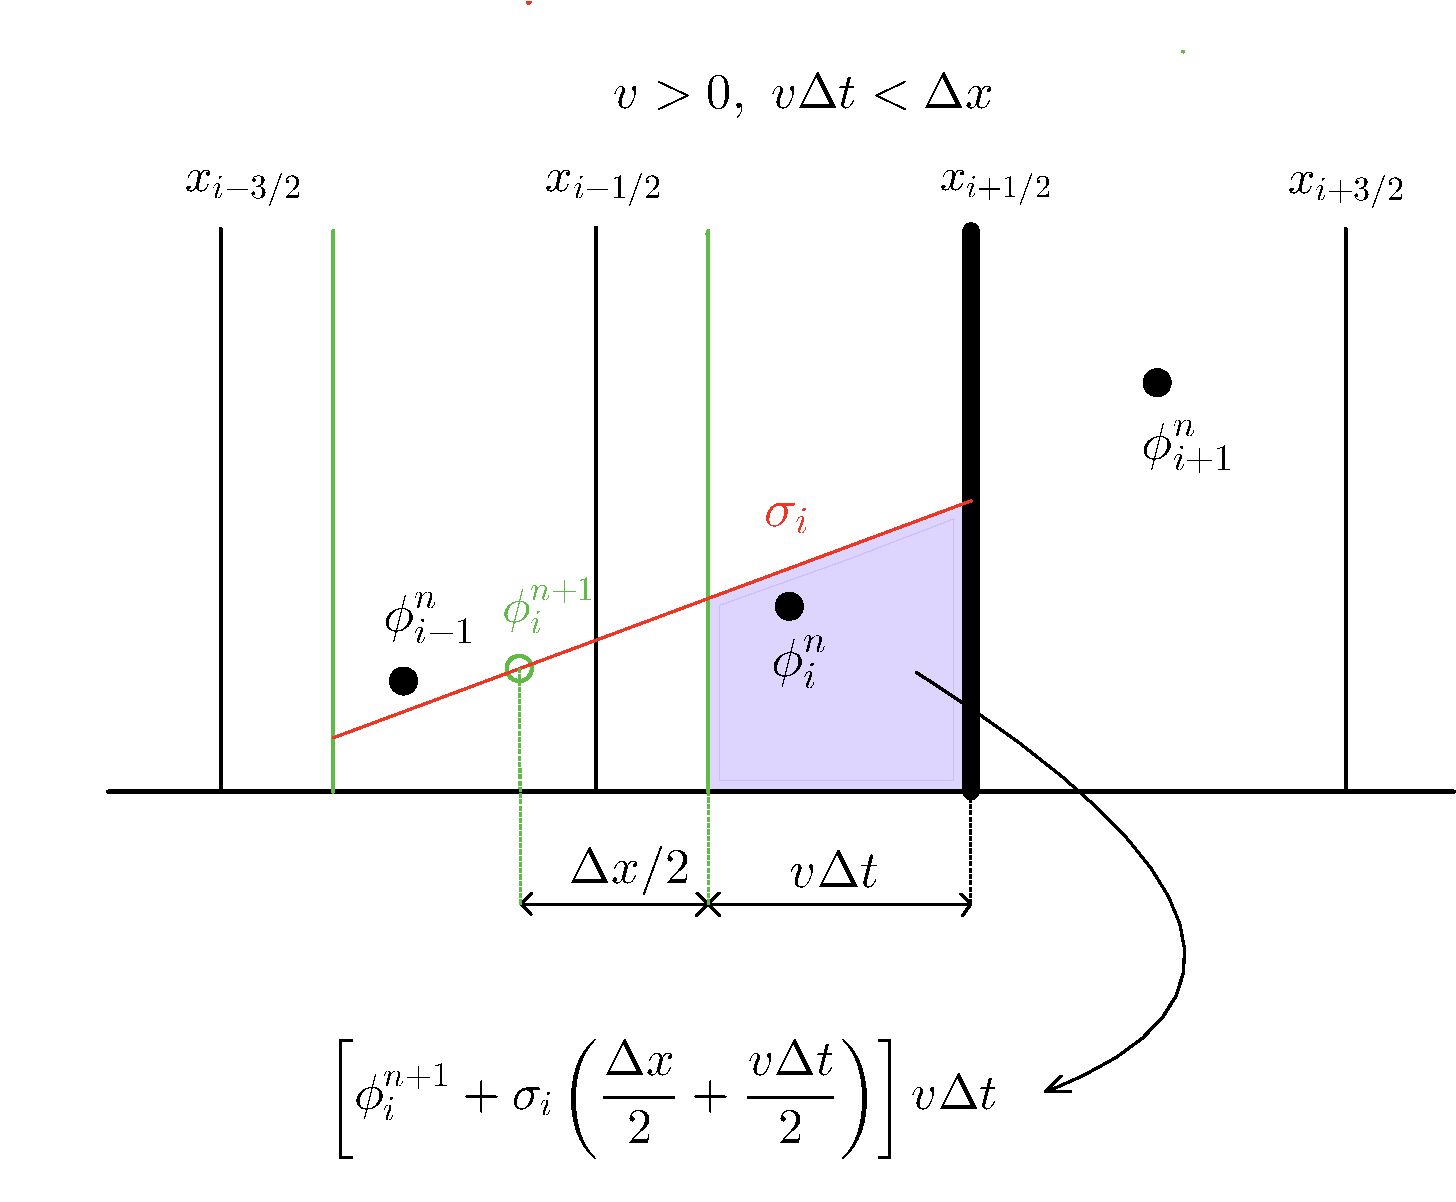
\includegraphics[width=\textwidth]{2nd-order-crop.pdf}
	\caption{Linear reconstruction with slope \(\sigma\)}
	\label{fig:linear-rec-1d}
\end{figure}
Let us begin with a linear reconstruction
\begin{equation}\label{eqn:linear-rec-poly}
    p(x) = \phi_{i}^{n+1} + \sigma_{i}\left( x - (x_{i}-v\Delta t) \right)
\end{equation}
with slope \(\sigma_{i}\) yielding second-order finite volume schemes, see Figure \ref{fig:linear-rec-1d}.
For \(v>0\), the quantity that flows through the face at \(x_{i+1/2}\) is simply the shaded area
\[ v\Delta t\left[
    \phi_{i}^{n+1} + \sigma_{i}\left( \frac{\Delta x}{2} + \frac{v\Delta t}{2} \right)
\right]. \]
Thus, the full update of the cell average
\begin{equation}
    \begin{split}
        \phi_{i}^{n+1}\Delta x
        =
        \phi_{i}^{n}\Delta x
        &-v\Delta t\left[
            \phi_{i}^{n+1} + \sigma_{i}\left( \frac{\Delta x}{2} + \frac{v\Delta t}{2} \right)
        \right]
        \\
        &+v\Delta t\left[
            \phi_{i-1}^{n+1} + \sigma_{i-1}\left( \frac{\Delta x}{2} + \frac{v\Delta t}{2} \right)
        \right].
    \end{split}
\end{equation}
Dividing by the cell width \(\Delta x\) and further simplifying we can write a general second-order implicit scheme
\begin{equation}\label{eqn:second-order-implicit}
    \begin{split}
        \phi_{i}^{n+1}
        &= \phi_{i}^{n} - c\left(
            \phi_{i}^{n+1}
            + \sigma_{i}\Delta x\frac{1+c}{2} - \phi_{i-1}^{n+1}
            -\sigma_{i-1}\Delta x\frac{1+c}{2} \right)
        \\
        &= \phi_{i}^{n} - c\left(
            \phi_{i}^{n+1}
            - \phi_{i-1}^{n+1}
            \right)
            -c\left(
            \sigma_{i} - \sigma_{i-1}
            \right)\Delta x\frac{1+c}{2},
    \end{split}
\end{equation}
where \(c = \frac{v\Delta t}{\Delta x}\) is the Courant number.
Different choices for the slope \(\sigma_{i}\)
yield different schemes studied in previous works,
see, e.g.,~\cite{2018_Frolkovic,2023_Frolkovic,2014_Mikula}.

Notice, that the linear reconstruction \eqref{eqn:linear-rec-poly} automatically satisfies the condition
\begin{equation}
    \frac{1}{\Delta x}
    \int_{x_{i-1/2}-v\Delta t}^{x_{i+1/2}-v\Delta t}
    p(x)\dd{x}
    = \phi_{i}^{n+1},
\end{equation}
since the line goes through the shifted center \(x_{i} - v\Delta t\). To compute the slope, we need one more condition. Thus, for example, our closest data to the face \(x_{i+1/2}\) is that the average value in the cell \(i\) is \(\phi_{i}^{n}\), so it is convenient to require the reconstruction to satisfy
\begin{equation}
    \frac{1}{\Delta x}
    \int_{x_{i+1/2}}^{x_{i+3/2}}
    p(x)\dd{x}
    =
    \frac{1}{\Delta x}
    \int_{x_{i+1/2}}^{x_{i+3/2}}
    \left[ \phi_{i}^{n+1} + \sigma_{i}
    \left( x - (x_{i}-v\Delta t) \right) \right]\dd{x}
    = \phi_{i}^{n}.
\end{equation}
The above integral equation is equivalent to requiring that the line goes through the center \(x_{i}\), yielding the slope
\begin{equation}
    \label{eqn:1point-slope}
    \sigma_{i} = \frac{\phi_{i}^{n} - \phi_{i}^{n+1}}{c \Delta x}.
\end{equation}
We can call it a 1 point scheme, since for computing the slope we use only 1 space coordinate \(x_{i}\), but the values are from different time levels.
Substituting the slope \eqref{eqn:1point-slope} to the general second-order implicit scheme \eqref{eqn:second-order-implicit} we get
\begin{equation}
    \begin{split}
        \phi_{i}^{n+1} &= \phi_{i}^{n} - c\left(
        \phi_{i}^{n+1}
        - \phi_{i-1}^{n+1}
        \right)
        -c\left(
        \sigma_{i} - \sigma_{i-1}
        \right)\Delta x\frac{1+c}{2},
        \\
        \phi_{i}^{n+1} &= \phi_{i}^{n} - c\left(
        \phi_{i}^{n+1}
        - \phi_{i-1}^{n+1}
        \right)
        -c\left(
            \frac{\phi_{i}^{n} - \phi_{i}^{n+1}}{c \Delta x}
            - \frac{\phi_{i-1}^{n} - \phi_{i-1}^{n+1}}{c \Delta x}
        \right)\Delta x\frac{1+c}{2},
    \end{split}
\end{equation}
yielding the system
\begin{equation}
    \label{eqn:1point-system}
    \begin{split}
        \left( -c + \frac{1+c}{2} \right)
        \phi_{i-1}^{n+1}
        + \left( 1 + c - \frac{1+c}{2} \right)
        \phi_{i}^{n+1}
        &=
        \frac{1+c}{2}\phi_{i-1}^{n}
        + \left( 1 - \frac{1+c}{2} \right)
        \phi_{i}^{n}
        \\
        \frac{1-c}{2}
        \phi_{i-1}^{n+1}
        + \frac{1+c}{2}
        \phi_{i}^{n+1}
        &=
        \frac{1+c}{2}\phi_{i-1}^{n}
        + \frac{1-c}{2}
        \phi_{i}^{n},
        \\
        \frac{1-c}{1+c}
        \phi_{i-1}^{n+1}
        + \phi_{i}^{n+1}
        &=
        \phi_{i-1}^{n}
        + \frac{1-c}{1+c}
        \phi_{i}^{n}.
    \end{split}
\end{equation}
Notice that the above scheme is exact for Courant number \(c = 1\).
Another choice, e.g., is if our linear reconstruction satisfies the integral equation
\begin{equation}
    \frac{1}{\Delta x}
    \int_{x_{i+1/2}}^{x_{i+3/2}}
    p(x)\dd{x}
    = \phi_{i+1}^{n},
\end{equation}
we get the slope
\begin{equation}
    \label{eqn:iioe-slope}
    \sigma_{i} = \frac{\phi_{i+1}^{n} - \phi_{i}^{n+1}}{(1+c)\Delta x}.
\end{equation}
Substituting \eqref{eqn:iioe-slope} to \eqref{eqn:second-order-implicit} yields the scheme
\begin{equation}\label{eqn:iioe-1d}
    \begin{split}
        \phi_{i}^{n+1}
        &= \phi_{i}^{n} - c\left(
            \phi_{i}^{n+1}
            - \phi_{i-1}^{n+1}
            \right)
            -c\left(
            \sigma_{i} - \sigma_{i-1}
            \right)\Delta x\frac{1+c}{2},
        \\
        &= \phi_{i}^{n} - c\left(
            \phi_{i}^{n+1}
            - \phi_{i-1}^{n+1}
            \right)
            -c\left(
                \frac{\phi_{i+1}^{n} - \phi_{i}^{n+1}}{(1+c)\Delta x}
                - \frac{\phi_{i}^{n} - \phi_{i-1}^{n+1}}{(1+c)\Delta x}
            \right)\Delta x\frac{1+c}{2},
        \\
        &= \phi_{i}^{n} - c\left(
            \phi_{i}^{n+1}
            - \phi_{i-1}^{n+1}
            \right)
            -\frac{c}{2}\left(
                \phi_{i+1}^{n} - \phi_{i}^{n+1}
                - (\phi_{i}^{n} - \phi_{i-1}^{n+1})
            \right),
        \\
        &= \phi_{i}^{n}
            -c\left(
                \frac{\phi_{i+1}^{n} + \phi_{i}^{n+1}}{2}
                - \frac{\phi_{i}^{n} + \phi_{i-1}^{n+1}}{2}
            \right),
    \end{split}
\end{equation}
which, as one can recognize, is the IIOE scheme for linear advection with constant speed in 1D \cite{2014_Mikula,2018_Frolkovic,2020_Ibolya_CONF}.
This yields a system
\begin{equation}
    \label{eqn:iioe-system}
    \begin{split}
        -\frac{c}{2}\phi_{i-1}^{n+1}
        +\left( 1 + \frac{c}{2} \right)
        \phi_{i}^{n+1}
        &=
        \left( 1 + \frac{c}{2} \right)
        \phi_{i}^{n}
        -\frac{c}{2}\phi_{i+1}^{n},
        \\
        -\frac{c}{2+c}\phi_{i-1}^{n+1}
        +\phi_{i}^{n+1}
        &=
        \phi_{i}^{n}
        -\frac{c}{2+c}\phi_{i+1}^{n}.
    \end{split}
\end{equation}
\subsection[]{A compact, third-order accurate, semi-implicit \\*piecewise-parabolic method}
\begin{figure}[H]
	\centering
	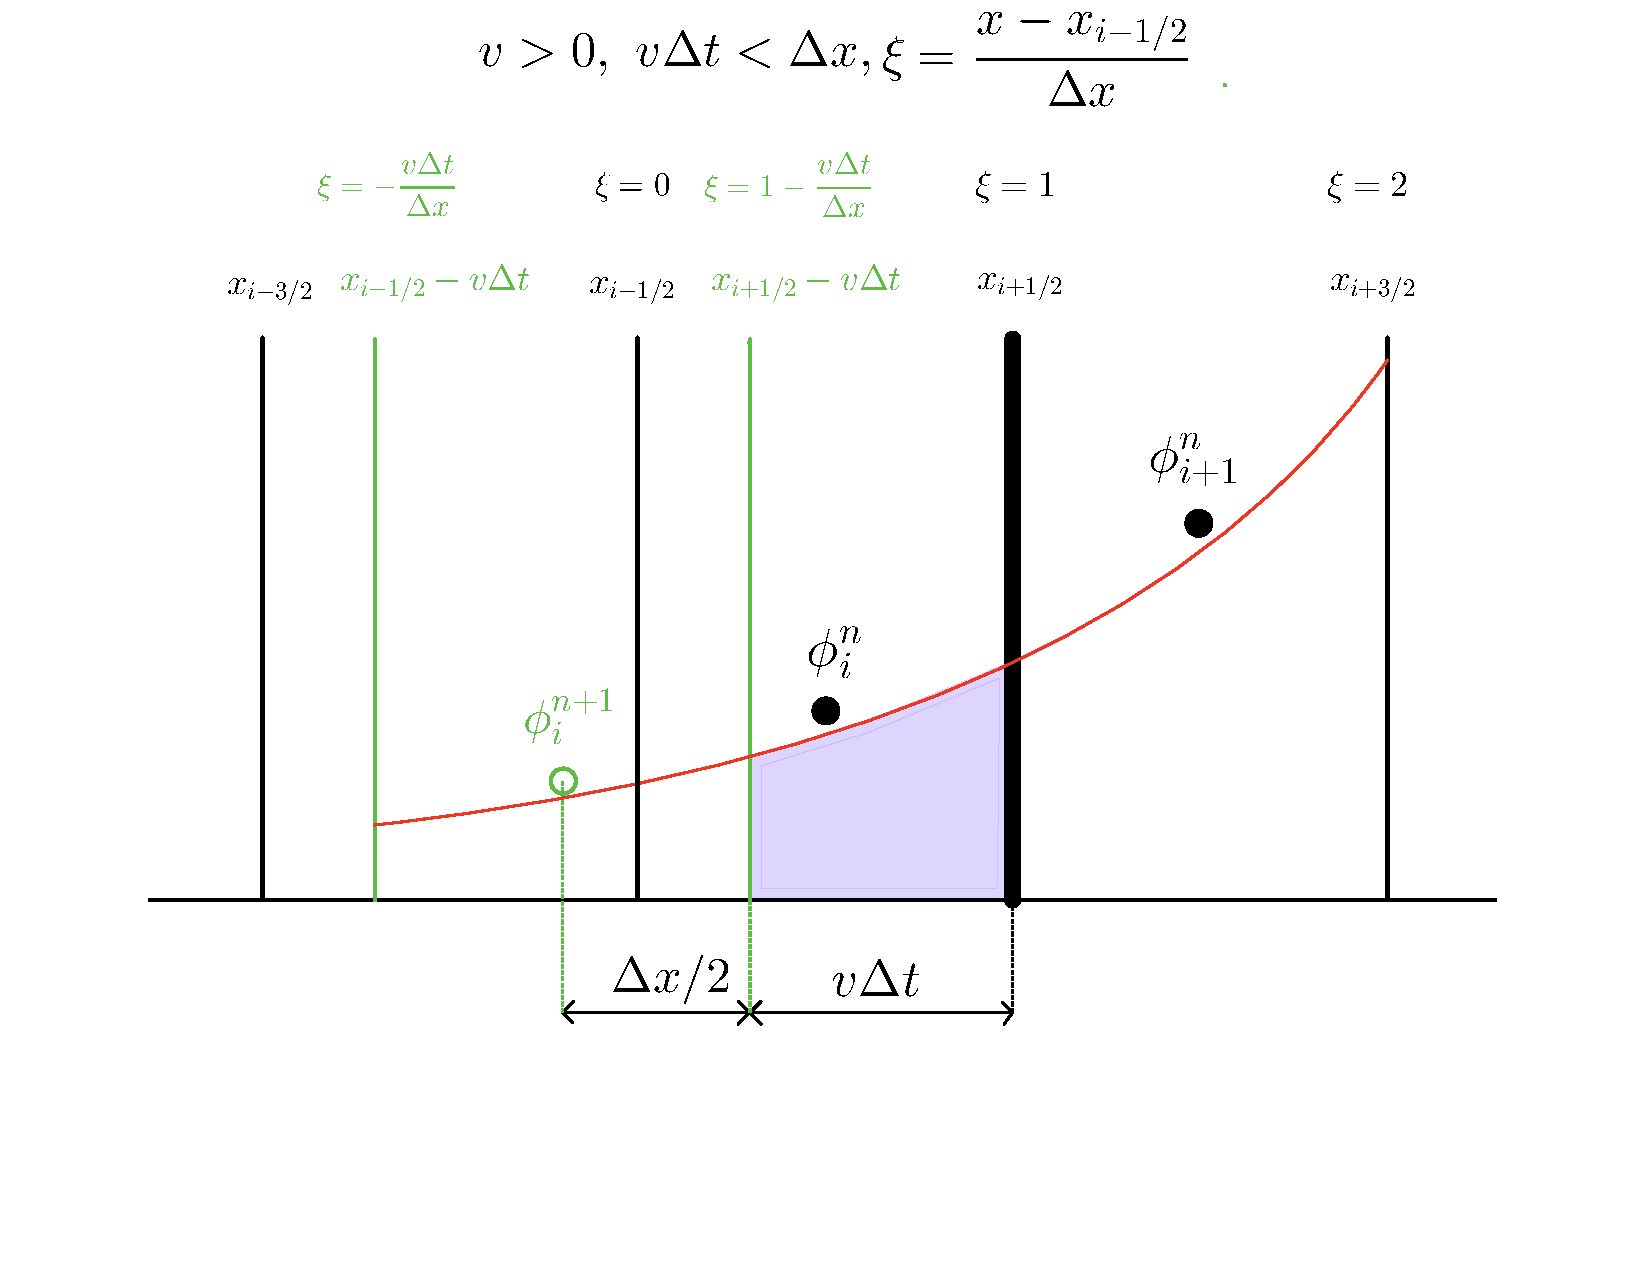
\includegraphics[width=\textwidth]{implicit-ppm-crop.pdf}
	\caption{Parabolic reconstruction}
	\label{fig:implicit-ppm}
\end{figure}
Instead of a linear reconstruction,
we can compute the average-flux at the face \(i+1/2\) using a piecewise-parabolic reconstruction using the cell averages \(\phi_{i+1}^{n}, \phi_{i}^{n}, \phi_{i}^{n+1}\). A second order polynomial can be written in the form
\begin{equation}
    p(x) = c_0 + c_1 x + c_2 x^2.
\end{equation}
In order to compute the three unknown coefficients, we require the reconstruction to satisfy the average equations in the appropriate intervals:
\begin{equation}
    \begin{split}
        \int_{x_{i+1/2}}^{x_{i+3/2}} p(x) \dd{x}
        &= \phi_{i+1}^{n}\Delta x,
        \\
        \int_{x_{i-1/2}}^{x_{i+1/2}} p(x) \dd{x}
        &= \phi_{i}^{n}\Delta x,
        \\
        \int_{x_{i-1/2} - c\Delta x}^{x_{i+1/2} - c\Delta x} p(x) \dd{x}
        &= \phi_{i}^{n+1}\Delta x.
    \end{split}
\end{equation}
For convenience, we can make a change of variables
\begin{equation}
    \xi = \frac{x-x_{i-1/2}}{\Delta x},
\end{equation}
and write the polynomial in a different form
\begin{equation}\label{eqn: parabola-xi}
    p(\xi) = c_0 + c_1\xi + c_2\xi^2.
\end{equation}
The integral equations become
\begin{equation}\label{eqn: parabola-integral-xi}
    \begin{split}
        \int_{1}^{2} p(\xi) \dd{\xi}
        &= \phi_{i+1}^{n},
        \\
        \int_{0}^{1} p(\xi) \dd{\xi}
        &= \phi_{i}^{n},
        \\
        \int_{-c}^{1-c} p(\xi) \dd{\xi}
        &= \phi_{i}^{n+1}.
    \end{split}
\end{equation}
Solving the equations yields
\begin{equation}
    \begin{split}
        c_0 &= \phi_{i}^{n+1}
        +\frac{1-3c}{6(1+c)}
        \left( \phi_{i+1}^{n}-\phi_{i}^{n} \right)
        +\frac{-2+3c+3c^2}{3(1+c)}
        \frac{\phi_{i}^{n}-\phi_{i}^{n+1}}{c},
        \\
        c_1 &=
        \frac{c-1}{1+c}
        \left( \phi_{i+1}^{n}-\phi_{i}^{n} \right)
        +\frac{2}{1+c}
        \frac{\phi_{i}^{n}-\phi_{i}^{n+1}}{c},
        \\
        c_2 &=
        \frac{1}{1+c}
        \left( \phi_{i+1}^{n}-\phi_{i}^{n} \right)
        -\frac{1}{1+c}
        \frac{\phi_{i}^{n}-\phi_{i}^{n+1}}{c}.
    \end{split}
\end{equation}
To get the average flux through the face \(x = x_{i+1/2}\), or \(\xi = 1\), we integrate
\begin{equation}
    \begin{split}
        \int_{x_{i+1/2}-c\Delta x}^{x_{i+1/2}} p(x) \dd{x}
        =
        \int_{1-c}^{1} p(\xi) \dd{\xi}
        &= c~c_0 + \frac{c(2-c)}{2}c_1 + \frac{c(3-3c+c^2)}{3}c_2
        \\
        &=c \left( \phi_{i}^{n+1}
        +\frac{1-c}{6}\left( \phi_{i+1}^{n}-\phi_{i}^{n} \right)
        +\frac{1+2c}{3}
        \frac{\phi_{i}^{n}-\phi_{i}^{n+1}}{c} \right)
        \\
        &= \frac{c-1}{3}\phi_{i}^{n+1}
        +\frac{2+3c+c^2}{6}\phi_{i}^{n}
        -\frac{c(c-1)}{6}\phi_{i+1}^{n}.
    \end{split}
\end{equation}
Also, evaluating the flux on the inflow face yields the system of equations
\begin{equation}
    \label{eqn:implicit-ppm-system}
    -\frac{1-c}{2+c}\phi_{i-1}^{n+1}
    +\phi_{i}^{n+1}
    =
    \frac{1+c}{2}\phi_{i-1}^{n}
    +(1-c)\phi_{i}^{n}
    -\frac{c(1-c)}{2(2+c)}\phi_{i+1}^{n}.
\end{equation}
The scheme is equivalent to a linear reconstruction, if the choice of the slope is
\begin{equation}
    \label{eqn:implicit-ppm-slope}
    \begin{split}
        \sigma_{i} = \frac{1-c}{3(1+c)}
        \frac{\phi_{i+1}^{n} - \phi_{i}^{n}}
        {\Delta x}
        + \frac{2(1+2c)}{3(1+c)}
        \frac{\phi_{i}^{n} - \phi_{i}^{n+1}}
        {c \Delta x}.
    \end{split}
\end{equation}
\section[]{Stabilization of second-order implicit schemes}
\subsection[]{The implicit upwind-range-condition}
\begin{figure}[H]
	\centering
	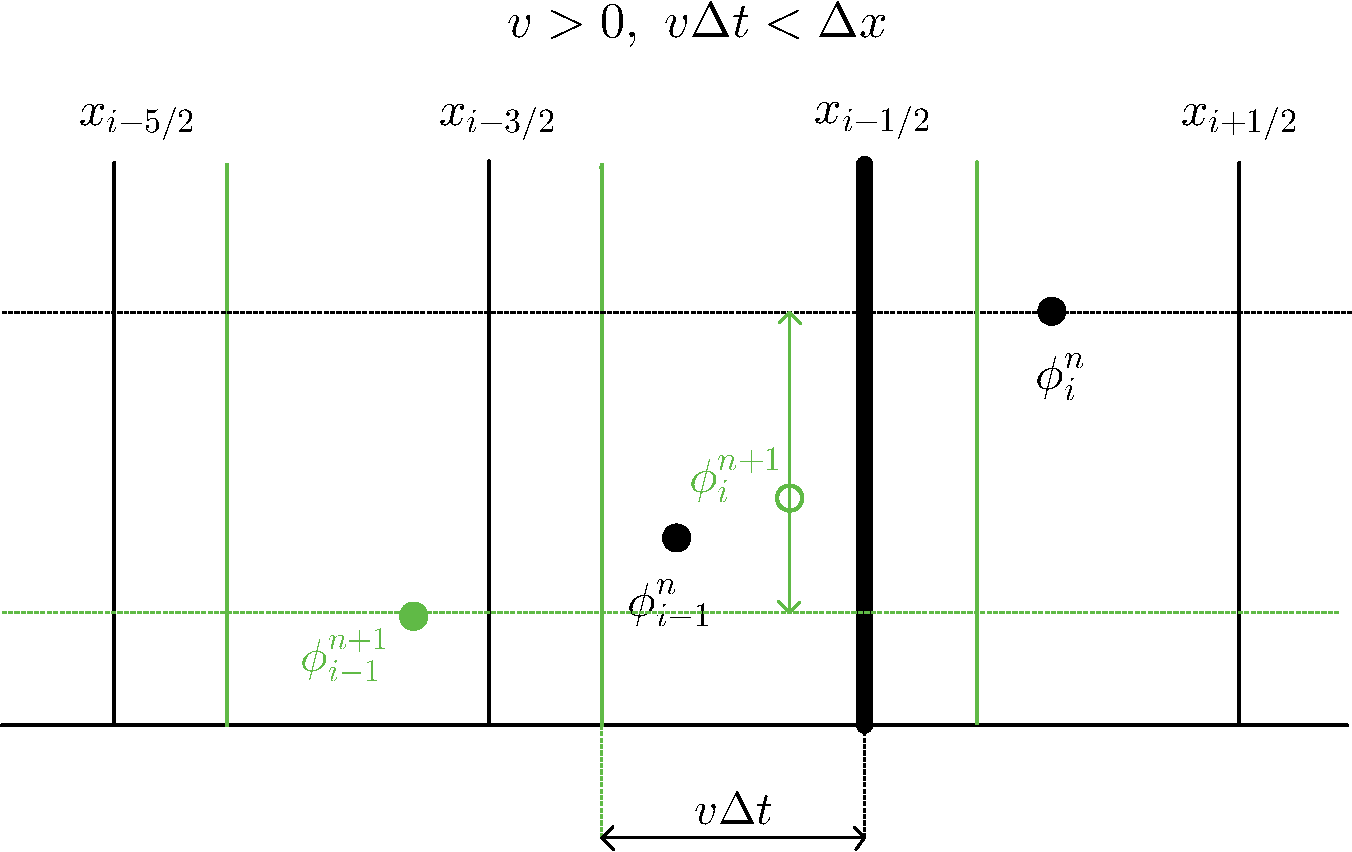
\includegraphics[width=\textwidth]{Implicit-urc-crop.pdf}
	\caption{Implicit upwind-range-condition}
	\label{fig:implicit-urc}
\end{figure}
In this section we construct stabilized schemes by requiring the updated cell average to lie between values \(\phi_{i-1}^{n+1},\phi_{i}^{n}\), thus
\begin{equation}\label{eqn:implicit-upwind-range-condition}
    \min\left( \phi_{i-1}^{n+1},\phi_{i}^{n} \right)
    \leq
    \phi_{i}^{n+1}
    \leq
    \max\left( \phi_{i-1}^{n+1},\phi_{i}^{n} \right),
\end{equation}
for \(c > 0\), see Figure \ref{fig:implicit-urc}. We can distinguish three cases:
\begin{enumerate}
    \item \(\phi_{i}^{n} > \phi_{i-1}^{n+1}:\)
        \[\min\left( \phi_{i-1}^{n+1},\phi_{i}^{n} \right) = \phi_{i-1}^{n+1},\quad
        \max\left( \phi_{i-1}^{n+1},\phi_{i}^{n} \right) = \phi_{i}^{n}.\]
        We can rewrite \eqref{eqn:implicit-upwind-range-condition} as
        \begin{equation*}
            \begin{split}
                \phi_{i-1}^{n+1}
                &\leq
                \phi_{i}^{n+1}
                \leq
                \phi_{i}^{n},
                \\
                0
                &\leq
                \phi_{i}^{n+1} - \phi_{i-1}^{n+1}
                \leq
                \phi_{i}^{n} - \phi_{i-1}^{n+1},
                \\
                0
                &\leq
                \frac{\phi_{i}^{n+1} - \phi_{i-1}^{n+1}}{\phi_{i}^{n} - \phi_{i-1}^{n+1}}
                \leq
                1.
            \end{split}
        \end{equation*}
    \item \(\phi_{i}^{n} < \phi_{i-1}^{n+1}:\)
        \[\min\left( \phi_{i-1}^{n+1},\phi_{i}^{n} \right) = \phi_{i}^{n},\quad
        \max\left( \phi_{i-1}^{n+1},\phi_{i}^{n} \right) = \phi_{i-1}^{n+1}.\]
        We can rewrite \eqref{eqn:implicit-upwind-range-condition} as
        \begin{equation*}
            \begin{split}
                \phi_{i}^{n}
                &\leq
                \phi_{i}^{n+1}
                \leq
                \phi_{i-1}^{n+1},
                \\
                \phi_{i}^{n} - \phi_{i-1}^{n+1}
                &\leq
                \phi_{i}^{n+1} - \phi_{i-1}^{n+1}
                \leq
                0,
                \\
                1
                &\geq
                \frac{\phi_{i}^{n+1} - \phi_{i-1}^{n+1}}{\phi_{i}^{n} - \phi_{i-1}^{n+1}}
                \geq
                0.
            \end{split}
        \end{equation*}
    \item \(\phi_{i}^{n} = \phi_{i-1}^{n+1}\), in which case we have\[\phi_{i}^{n} = \phi_{i-1}^{n+1} = \phi_{i}^{n+1}.\]
\end{enumerate}
Notice, that for the first two cases, where \(\phi_{i}^{n} \neq \phi_{i-1}^{n+1}\) we can simply require
\begin{equation}\label{eqn:upwind-range-simpler}
    0
    \leq
    \frac{\phi_{i}^{n+1} - \phi_{i-1}^{n+1}}{\phi_{i}^{n} - \phi_{i-1}^{n+1}}
    \leq
    1
\end{equation}
instead of \eqref{eqn:implicit-upwind-range-condition} to simplify the analysis.
The condition above can be interpreted as the upwind range condition\cite{1998_Laney_BOOK},
data compatibility condition \cite{2009_Toro_BOOK}, upwind monotonic property \cite{1989_Huynh_CONF}, local boundedness property \cite{1982_Roe,1997_Thuburn} for implicit schemes.
The idea is that the solution travels along characteristics and this value is always bounded by its neighbors in space-time. In the case of well established explicit schemes, requiring a scheme to satisfy the upwind-range property is equivalent to requiring a scheme to be TVD \cite{1997_Thuburn}. However, as it was also pointed out in \cite{1997_Thuburn}, this condition is a more straightforward local condition, which makes it also more straightforward to extend to more complicated equations even in higher dimensions, than the TVD condition. Not to mention the results of LeVeque and Goodman, \cite{1985_LeVeque_CONF}, where they prove, that a two-dimensional TVD scheme can be at most first-order accurate.

Notice that min and max is a combination of values from both time steps \(n, n+1\).
This distinguishes the implicit upwind-range property from the explicit one.
In the explicit case, the min and max are chosen only from the values at the current time step \(n\).

First, we show that if a scheme satisfies the upwind-range-condition, then it is also total variation non-increasing, which property is often referred to as TVD.
In order to show this, first notice that if the new cell average \(\phi_{i}^{n+1}\) lies
between the values \(\phi_{i-1}^{n+1}, \phi_{i}^{n}\), then it can be written as a convex combination of the two
\begin{equation}\label{eqn:convex-combination}
    \phi_{i}^{n+1} =
    k_{i}\phi_{i}^{n} + (1-k_{i})\phi_{i-1}^{n+1},
\end{equation}
for some \(0 \leq k_{i} \leq 1\).

If \(k_{i} = 0\), then
\[
    \phi_{i}^{n+1} = \phi_{i-1}^{n+1},
\]
thus, if \(\phi_{i-1}^{n+1}\), the update does certainly not create new extrema.

For \(k_{i} > 0\), we can recast the above convex combination to a conservation form
\begin{equation}\label{eqn:convex-combination-conservative}
    \begin{split}
        \phi_{i}^{n+1}
        &=
        k_{i}\phi_{i}^{n} + (1-k_{i})\phi_{i-1}^{n+1},
        \\
        \frac{1}{k_{i}}\phi_{i}^{n+1}
        &=
        \phi_{i}^{n} + \frac{1-k_{i}}{k_{i}}\phi_{i-1}^{n+1},
        \\
        \frac{1}{k_{i}}\phi_{i}^{n+1} + \phi_{i}^{n+1} - \phi_{i}^{n+1}
        &=
        \phi_{i}^{n} + \frac{1-k_{i}}{k_{i}}\phi_{i-1}^{n+1},
        \\
        \phi_{i}^{n+1} + \frac{1-k_{i}}{k_{i}}\phi_{i}^{n+1}
        &=
        \phi_{i}^{n} + \frac{1-k_{i}}{k_{i}}\phi_{i-1}^{n+1},
        \\
        \phi_{i}^{n+1}
        &=
        \phi_{i}^{n} - \frac{1-k_{i}}{k_{i}}\left( \phi_{i}^{n+1} - \phi_{i-1}^{n+1} \right).
    \end{split}
\end{equation}
Notice that if \(0 < k_{i} \leq 1\), then \( \frac{1-k_{i}}{k_{i}} > 0\), which is sufficient for a scheme to be TVD, see, e.g.,~\cite{2007_Duraisamy,2023_Frolkovic}.

We need a few definitions, that will make some of our formulations simpler, where we want to enforce bounds, see, e.g., \cite{1989_Huynh_CONF,1993_Huynh}.

Let \(I(z_{1}, \dots, z_{k})\) be the smallest closed interval containing \(z_{1}, \dots, z_{k}\),
thus,
\begin{equation}
    I(z_{1}, \dots, z_{k})
    = \left[\min(z_{1}, \dots, z_{k}),
    \max(z_{1}, \dots, z_{k})\right].
\end{equation}
The \(\mbox{median}\) of three numbers is the one, which lies between the other two.
In order to define the median function, first we need a definition of the minmod function of two variables(see, e.g., \cite{1993_Huynh}):
% \begin{equation}
%     \mbox{minmod}(a,b) =
%     \begin{cases}
%         a & \text{if}\ |a| < |b|\ \text{and}\ ab > 0, \\
%         b & \text{if}\ |b| < |a|\ \text{and}\ ab > 0, \\
%         0 & \text{if}\ ab < 0.
%     \end{cases}
% \end{equation}
\begin{equation}
    \mbox{minmod}(a,b) =
    \begin{cases}
        \mbox{sgn}(a) \min(|a|,|b|) & \text{if}\ ab > 0, \\
        0 & \text{otherwise}.
    \end{cases}
\end{equation}
Then, the median function of 3 variables, as in \cite{1989_Huynh_CONF,1993_Huynh}, can be defined
\begin{equation}
    \begin{split}
        \mbox{median}(a,b,c)
        &= a + \mbox{minmod}\left( b - a, c - a \right)
        \\
        &= b + \mbox{minmod}\left( a - b, c - b \right).
    \end{split}
\end{equation}

It is important to observe that the \(\mbox{median}(x,y,z)\) lies in the interval defined by any other two of the three arguments, e.g.,
\begin{equation}
    \mbox{median}(x,y,z) \in I(y,z),\ \text{or}\
    \mbox{median}(x,y,z) \in I(x,z).
\end{equation}
Also, \(\mbox{median}(z_{1}, z_{2},z_{3}, z_{4},z_{5})\) lies in the interval defined by any three of the five arguments, e.g.,
\begin{equation}
    \mbox{median}(z_{1},\dots,z_{5}) \in I(z_{1},z_{4}, z_{3}).
\end{equation}
Using the definitions above, the upwind-range condition \eqref{eqn:upwind-range-simpler} can be written in a convenient way by requiring
\begin{equation}
    \phi_{i}^{n+1}\in I(\phi_{i-1}^{n+1}, \phi_{i}^{n}).
\end{equation}
\subsection[]{Second-order implicit TVD schemes}
Now we describe how we can construct schemes satisfying the upwind-range condition by choosing the slope appropriately.
We can solve
\begin{equation}
    \phi_{i}^{n+1}
    = \phi_{i}^{n} - c\left(
        \phi_{i}^{n+1}
        - \phi_{i-1}^{n+1}
        \right)
        -c\left(
        \sigma_{i} - \sigma_{i-1}
        \right)\Delta x\frac{1+c}{2},
\end{equation}
for the new cell average to obtain
\begin{equation}\label{eqn: second order implicit - solution}
    \phi_{i}^{n+1} =
    \frac{\phi_{i}^{n} +
    c~\phi_{i-1}^{n+1}}{1+c}
    -\frac{c}{2}\left(
        \sigma_{i} - \sigma_{i-1}
        \right)\Delta x.
\end{equation}
\begin{remark}
    Notice, that in the schemes we describe, the slope \(\sigma_{i}\) can also contain terms involving \(\phi_{i}^{n+1}\).
\end{remark}
Substituting to the upwind-range condition \eqref{eqn:upwind-range-simpler} we get
\begin{equation}
    \begin{split}\label{eqn: urc-all c-necessary}
        0
        &\leq
        \frac{\phi_{i}^{n+1} - \phi_{i-1}^{n+1}}
        {\phi_{i}^{n} - \phi_{i-1}^{n+1}}
        \leq
        1,
        \\
        0
        &\leq
        \frac{
        \frac{\phi_{i}^{n} +
        c~\phi_{i-1}^{n+1}}{1+c}
        -\frac{c}{2}\left(
            \sigma_{i} - \sigma_{i-1}
            \right)\Delta x - \phi_{i-1}^{n+1}}{\phi_{i}^{n} - \phi_{i-1}^{n+1}}
        \leq
        1,
        \\
        0
        &\leq
        \frac{
        \frac{\phi_{i}^{n} - \phi_{i-1}^{n+1}}{1+c}
        -\frac{c}{2}\left(
            \sigma_{i} - \sigma_{i-1}
            \right)\Delta x}{\phi_{i}^{n} - \phi_{i-1}^{n+1}}
        \leq
        1,
        \\
        0
        &\leq
        \frac{1}{1+c}
        -\frac{c}{2}
        \frac{\sigma_{i}\Delta x}
        {\phi_{i}^{n} - \phi_{i-1}^{n+1}}
        +\frac{c}{2}
        \frac{\sigma_{i-1}\Delta x}
        {\phi_{i}^{n} - \phi_{i-1}^{n+1}}
        \leq
        1.
    \end{split}
\end{equation}
\begin{figure}[H]
	\centering
	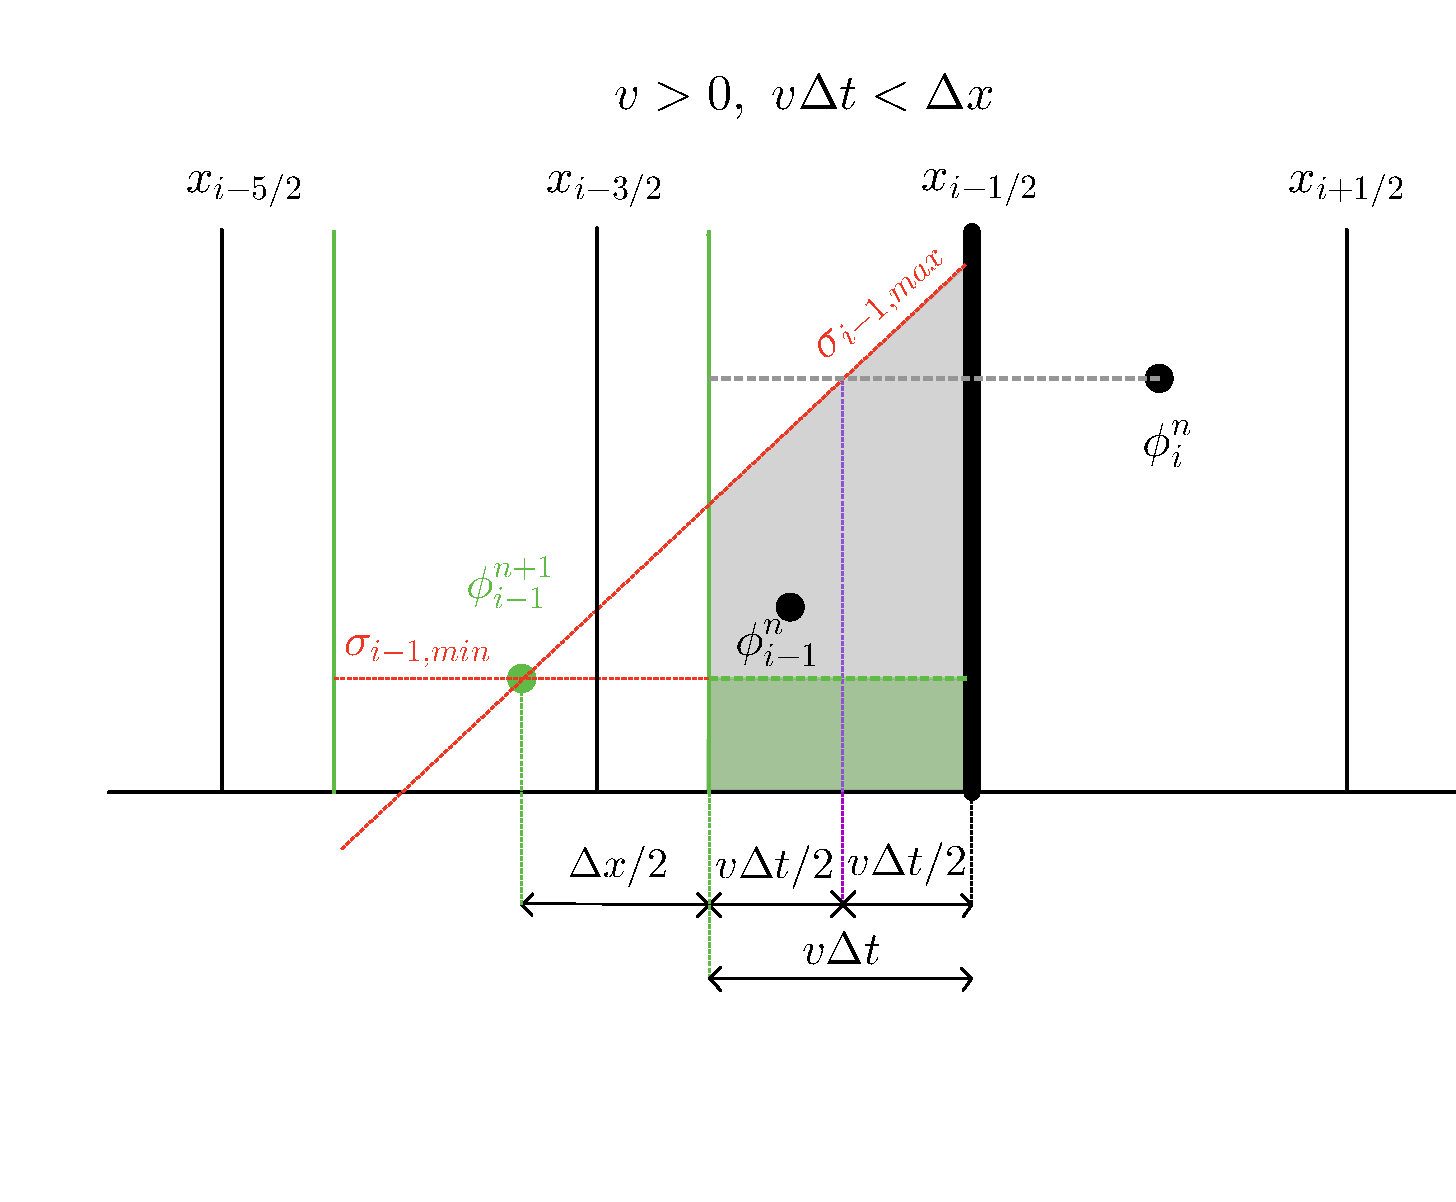
\includegraphics[width=\textwidth]{Slope-bounds-crop.pdf}
	\caption{Bounds for the slope}
	\label{fig:slope-bounds-implicit-1d}
\end{figure}
We require that the flux through the face at \(x = x_{i-1/2}\) be bounded by the downwind flux, \(v\Delta t\ \phi_{i}^{n}\), and the implicit upwind flux, \(v\Delta t\ \phi_{i-1}^{n+1}\), see Figure \ref{fig:slope-bounds-implicit-1d}. Thus, we write
\begin{equation}\label{eqn: urc-all c-bounded slope}
    \begin{split}
        v\Delta t\min(\phi_{i-1}^{n+1},\phi_{i}^{n})
        \leq
        v\Delta t
        \left[
            \phi_{i-1}^{n+1}
            +\sigma_{i-1}\left(
                \frac{\Delta x}{2} + \frac{v\Delta t}{2}
                \right)
        \right]
        &\leq
        v\Delta t\max(\phi_{i-1}^{n+1},\phi_{i}^{n}),
        \\
        \min(\phi_{i-1}^{n+1},\phi_{i}^{n})
        \leq
        \phi_{i-1}^{n+1}
        +\sigma_{i-1} \Delta x \frac{1+c}{2}
        &\leq
        \max(\phi_{i-1}^{n+1},\phi_{i}^{n}).
    \end{split}
\end{equation}
Notice, that this is the same upwind-range condition, as for the new cell average \eqref{eqn:upwind-range-simpler}. Thus, the above condition is equivalent to requiring
\begin{equation}
    \label{eqn:slope-bounds}
    \begin{split}
        0
        \leq
        \frac{\phi_{i-1}^{n+1}
        +\sigma_{i-1}\frac{1+c}{2}\Delta x
        - \phi_{i-1}^{n+1}}{\phi_{i}^{n} - \phi_{i-1}^{n+1}}
        &\leq
        1,
        \\
        0
        \leq
        \frac{1+c}{2}
        \frac{\sigma_{i-1}\Delta x}
        {\phi_{i}^{n} - \phi_{i-1}^{n+1}}
        &\leq
        1,
        \\
        0
        \leq
        \frac{c}{2}
        \frac{\sigma_{i-1}\Delta x}
        {\phi_{i}^{n} - \phi_{i-1}^{n+1}}
        &\leq
        \frac{c}{1+c},
        \\
        0
        \leq
        \frac{\sigma_{i-1}\Delta x}
        {\phi_{i}^{n} - \phi_{i-1}^{n+1}}
        &\leq
        \frac{2}{1+c}.
    \end{split}
\end{equation}
The slopes must satisfy
\begin{equation}
    \label{eqn:slope-necessary}
    \begin{split}
        0
        &\leq
        \frac{1}{1+c}
        -\frac{c}{2}
        \frac{\sigma_{i}\Delta x}
        {\phi_{i}^{n} - \phi_{i-1}^{n+1}}
        +\frac{c}{2}
        \frac{\sigma_{i-1}\Delta x}
        {\phi_{i}^{n} - \phi_{i-1}^{n+1}}
        \leq
        1,
        \\
        -\left(\frac{1}{1+c}
        + \frac{c}{2}
        \frac{\sigma_{i-1}\Delta x}
        {\phi_{i}^{n} - \phi_{i-1}^{n+1}}\right)
        &\leq
        -\frac{c}{2}
        \frac{\sigma_{i}\Delta x}
        {\phi_{i}^{n} - \phi_{i-1}^{n+1}}
        \leq
        1-\left(\frac{1}{1+c}
        + \frac{c}{2}
        \frac{\sigma_{i-1}\Delta x}
        {\phi_{i}^{n} - \phi_{i-1}^{n+1}}\right),
        \\
        -\left(\frac{1}{1+c}
        + \frac{c}{2}
        \frac{\sigma_{i-1}\Delta x}
        {\phi_{i}^{n} - \phi_{i-1}^{n+1}}\right)
        &\leq
        -\frac{c}{2}
        \frac{\sigma_{i}\Delta x}
        {\phi_{i}^{n} - \phi_{i-1}^{n+1}}
        \leq
        \frac{c}{1+c}
        - \frac{c}{2}
        \frac{\sigma_{i-1}\Delta x}
        {\phi_{i}^{n} - \phi_{i-1}^{n+1}},
        \\
        \frac{1}{1+c}
        + \frac{c}{2}
        \frac{\sigma_{i-1}\Delta x}
        {\phi_{i}^{n} - \phi_{i-1}^{n+1}}
        &\geq
        \frac{c}{2}
        \frac{\sigma_{i}\Delta x}
        {\phi_{i}^{n} - \phi_{i-1}^{n+1}}
        \geq
        \frac{c}{2}
        \frac{\sigma_{i-1}\Delta x}
        {\phi_{i}^{n} - \phi_{i-1}^{n+1}}
        -\frac{c}{1+c},
        \\
        \frac{\sigma_{i-1}\Delta x}
        {\phi_{i}^{n} - \phi_{i-1}^{n+1}}
        -\frac{2}{1+c}
        &\leq
        \frac{\sigma_{i}\Delta x}
        {\phi_{i}^{n} - \phi_{i-1}^{n+1}}
        \leq
        \frac{2}{c(1+c)}
        + \frac{\sigma_{i-1}\Delta x}
        {\phi_{i}^{n} - \phi_{i-1}^{n+1}}.
    \end{split}
\end{equation}
Also, from \eqref{eqn: urc-all c-bounded slope}, we have
\begin{equation}
    0
    \leq
    \frac{c}{2}
    \frac{\sigma_{i}\Delta x}
    {\phi_{i+1}^{n} - \phi_{i}^{n+1}}
    \leq
    \frac{c}{1+c}.
\end{equation}
Let us define the intervals
\begin{equation}
    I_{1}=I\left(
        \sigma_{i-1}
        -2\frac{\phi_{i}^{n} - \phi_{i-1}^{n+1}}
        {(1+c)\Delta x},
        ~\sigma_{i-1}
        +\frac{2}{c}
        \frac{\phi_{i}^{n} - \phi_{i-1}^{n+1}}
        {(1+c)\Delta x}
    \right),\
    I_{2} = I\left(
        0,
        ~2\frac{\phi_{i+1}^{n} - \phi_{i}^{n+1}}{(1+c)\Delta x}
    \right),
\end{equation}
then the slope must lie in the intersection
\begin{equation}
    \sigma_{i} \in I_{1} \cap I_{2}.
\end{equation}
Using \eqref{eqn:slope-bounds} and \eqref{eqn:slope-necessary}, we can see that
\begin{equation}
        \frac{\sigma_{i-1}\Delta x}
        {\phi_{i}^{n} - \phi_{i-1}^{n+1}}
        -\frac{2}{1+c}
        \leq
        0
        \leq
        \frac{2}{c(1+c)}
        + \frac{\sigma_{i-1}\Delta x}
        {\phi_{i}^{n} - \phi_{i-1}^{n+1}},
\end{equation}
which implies that \(0 \in I_{1}\).

Now we discuss how to compute a particular slope. Let us have a slope from a high-order reconstruction of our choice denoted as \(\sigma_{i}^{HO}\). We want to use this slope as much as possible. So, for example, if
\begin{equation}
    \sigma_{i}^{HO} \in I_{1} \cap I_{2}
    \Rightarrow
    \sigma_{i} = \sigma_{i}^{HO},
\end{equation}
otherwise the slope takes the value of one of the bounds from the interval \(I_{1} \cap I_{2}\).
Let
\begin{equation}
    \sigma^{(1)}
    = \mbox{median}\left(
        \sigma_{i-1}
        -2\frac{\phi_{i}^{n} - \phi_{i-1}^{n+1}}
        {(1+c)\Delta x},
        ~\sigma_{i-1}
        +\frac{2}{c}
        \frac{\phi_{i}^{n} - \phi_{i-1}^{n+1}}
        {(1+c)\Delta x},
        ~2\frac{\phi_{i+1}^{n} - \phi_{i}^{n+1}}{(1+c)\Delta x}
    \right),
\end{equation}
then, in order to satisfy the stability condition \eqref{eqn:upwind-range-simpler}, the slope of our reconstruction has to be
\begin{equation}
    \label{eqn:monotone-slope}
    \sigma_{i} = \mbox{minmod}\left(
        \sigma_{i}^{HO},\sigma^{(1)}
    \right).
\end{equation}
\begin{proof}
    (NOT COMPLETE!!!)
    The above equation \eqref{eqn:monotone-slope} can be equivalently written as
    \[
        \sigma_{i} = \mbox{median}\left(
            0,\sigma_{i}^{HO},\sigma^{(1)}
        \right),
    \]
    which implies, using a property of the median function, that
    \[\sigma_{i} \in I(0,\sigma^{(1)}).\]
    We can see, that both
    \[
        \sigma^{(1)} \in I_{1} \quad \text{and}\quad
        0 \in I_{1},
    \]
    thus, we conclude that \(\sigma_{i} \in I_{1}\).
    \((\textcolor{red}{\sigma_{i} \in I_{1}!!!})\)
    Again, using a property of the median function,
    we have
    \[
        \sigma^{(1)}
        \in
        I\left(
        \sigma_{i-1}
        -2\frac{\phi_{i}^{n} - \phi_{i-1}^{n+1}}
        {(1+c)\Delta x},
        ~2\frac{\phi_{i+1}^{n} - \phi_{i}^{n+1}}{(1+c)\Delta x}
        \right)
    \]
    or
    \[
        \sigma^{(1)}
        \in
        I\left(
        \sigma_{i-1}
        +\frac{2}{c}
        \frac{\phi_{i}^{n} - \phi_{i-1}^{n+1}}
        {(1+c)\Delta x},
        ~2\frac{\phi_{i+1}^{n} - \phi_{i}^{n+1}}{(1+c)\Delta x}
        \right)
    \]
\end{proof}
Using \eqref{eqn: urc-all c-necessary} and \eqref{eqn: urc-all c-bounded slope}, we can also derive sufficient condition for the slope \(\sigma_{i}\)
\begin{equation}\label{eqn: urc-all c- sufficient}
    \begin{split}
        0
        \leq
        \frac{1}{1+c}
        -\frac{c}{2}
        \frac{\sigma_{i}\Delta x}
        {\phi_{i}^{n} - \phi_{i-1}^{n+1}}
        &\leq
        1 - \frac{c}{1+c},
        \\
        0
        \leq
        \frac{1}{1+c}
        -\frac{c}{2}
        \frac{\sigma_{i}\Delta x}
        {\phi_{i}^{n} - \phi_{i-1}^{n+1}}
        &\leq
        \frac{1}{1+c},
        \\
        0
        \leq
        \frac{\sigma_{i}\Delta x}
        {\phi_{i}^{n} - \phi_{i-1}^{n+1}}
        &\leq
        \frac{2}{c}
        \frac{1}{1+c},
        % \\
        % |\sigma_{i}|
        % &\leq
        % \frac{2}{c}
        % \frac{|\phi_{i}^{n} - \phi_{i-1}^{n+1}|}
        % {(1+c)\Delta x}.
    \end{split}
\end{equation}
so the slope must lie in
\begin{equation}
    \label{eqn:slope-sufficient}
    \sigma_{i}
    \in
    I\left(
        0,
        \frac{2}{c}
        \frac{\phi_{i}^{n} - \phi_{i-1}^{n+1}}{1+c}
    \right)
    \cap
    I\left(
        0,
        ~2\frac{\phi_{i+1}^{n} - \phi_{i}^{n+1}}{(1+c)\Delta x}
    \right)
\end{equation}
% \begin{equation}
%     |\sigma_{i}|
%     \leq
%     \min \left(
%         \frac{2}{c}
%         \frac{|\phi_{i}^{n} - \phi_{i-1}^{n+1}|}
%         {(1+c)\Delta x},
%         2\frac{|\phi_{i+1}^{n} - \phi_{i}^{n+1}|}
%         {(1+c)\Delta x}
%     \right).
% \end{equation}
\begin{remark}
    We can derive similar schemes appearing in \cite{2023_Frolkovic} by writing the slope as a convex combination
    \begin{equation}
        \begin{split}
            \sigma_{i} &=
            (1-\omega_{i})
            \frac{\phi_{i+1}^{n}-\phi_{i}^{n+1}}
            {(1+c)\Delta x}
            + \omega_{i}
            \frac{\phi_{i}^{n} - \phi_{i-1}^{n+1}}
            {(1+c)\Delta x},
            \\
            &=
            \left( 1 - \omega_{i} + \omega_{i}r_i \right)
            \frac{\phi_{i+1}^{n}-\phi_{i}^{n+1}}
            {(1+c)\Delta x},
            \\
            &=
            \Psi_{i}
            \frac{\phi_{i+1}^{n}-\phi_{i}^{n+1}}
            {(1+c)\Delta x},
        \end{split}
    \end{equation}
where
\begin{equation}
    0 \leq \omega_{i} \leq 1,\quad
    \Psi_{i} = \Psi_{i}(r_{i}) =
    \left( 1 - \omega_{i} + \omega_{i}r_{i} \right),
    \quad
    r_{i} = \frac{\phi_{i}^{n} - \phi_{i-1}^{n+1}}
    {\phi_{i+1}^{n}-\phi_{i}^{n+1}}.
\end{equation}
Substituting the new form of the slopes we get
\begin{equation}\label{eqn: Frolkovic - necessary condition}
    \begin{split}
        0
        &\leq
        \frac{1}{1+c}
        -\frac{c}{2}
        \frac{\sigma_{i}\Delta x}
        {\phi_{i}^{n} - \phi_{i-1}^{n+1}}
        +\frac{c}{2}
        \frac{\sigma_{i-1}\Delta x}
        {\phi_{i}^{n} - \phi_{i-1}^{n+1}}
        \leq
        1,
        \\
        0
        &\leq
        \frac{1}{1+c}
        -\frac{c}{2}
        \frac{
            \Psi_{i}
            \frac{\phi_{i+1}^{n}-\phi_{i}^{n+1}}
            {(1+c)\Delta x}\Delta x}
            {\phi_{i}^{n} - \phi_{i-1}^{n+1}}
        +\frac{c}{2}
        \frac{
            \Psi_{i-1}
            \frac{\phi_{i}^{n}-\phi_{i-1}^{n+1}}
            {(1+c)\Delta x}\Delta x}
            {\phi_{i}^{n} - \phi_{i-1}^{n+1}}
        \leq
        1,
        \\
        0
        &\leq
        \frac{1}{1+c}
        -\frac{c}{2(1+c)}
        \frac{\Psi_{i}}{r_{i}}
        +\frac{c}{2(1+c)}
        \Psi_{i-1}
        \leq
        1.
    \end{split}
\end{equation}
Also, we consider similar bounds as before \eqref{eqn:slope-bounds}
\begin{equation}
    \begin{split}\label{eqn: Frolkovic - psi bounds}
        0
        &\leq
        \frac{\phi_{i-1}^{n+1}
        +\sigma_{i-1}\frac{1+c}{2}\Delta x
        - \phi_{i-1}^{n+1}}{\phi_{i}^{n} - \phi_{i-1}^{n+1}}
        \leq
        1,
        \\
        0
        &\leq
        \frac{\phi_{i-1}^{n+1}
        +\Psi_{i-1}
        \frac{\phi_{i}^{n}-\phi_{i-1}^{n+1}}
        {(1+c)\Delta x}\frac{1+c}{2}\Delta x
        - \phi_{i-1}^{n+1}}{\phi_{i}^{n} - \phi_{i-1}^{n+1}}
        \leq
        1,
        \\
        0
        &\leq
        \Psi_{i-1}
        \leq
        2.
    \end{split}
\end{equation}
(This condition, however, differs a little from the one appearing in \cite{2023_Frolkovic}, where they require \(-1 \leq \Psi_{i-1} \leq 2\)).

If \(\Psi_{i-1}\) is available, then
\begin{equation}
    \begin{split}
        -\left(
            \frac{1}{1+c} + \frac{c}{2(1+c)}\Psi_{i-1} \right)
        &\leq
        -\frac{c}{2(1+c)}
        \frac{\Psi_{i}}{r_{i}}
        \leq
        1-\left(
            \frac{1}{1+c} + \frac{c}{2(1+c)}\Psi_{i-1} \right),
        \\
        -\left(
            \frac{1}{1+c} + \frac{c}{2(1+c)}\Psi_{i-1} \right)
        &\leq
        -\frac{c}{2(1+c)}
        \frac{\Psi_{i}}{r_{i}}
        \leq
        \frac{c}{1+c} - \frac{c}{2(1+c)}\Psi_{i-1},
        \\
        \frac{1}{1+c} + \frac{c}{2(1+c)}\Psi_{i-1}
        &\geq
        \frac{c}{2(1+c)}
        \frac{\Psi_{i}}{r_{i}}
        \geq
        \frac{c}{2(1+c)}\Psi_{i-1} - \frac{c}{1+c},
        \\
        \frac{2}{c} + \Psi_{i-1}
        &\geq
        \frac{\Psi_{i}}{r_{i}}
        \geq
        \Psi_{i-1} - 2,
        \\
        \Psi_{i-1} - 2
        &\leq
        \frac{\Psi_{i}}{r_{i}}
        \leq
        \frac{2}{c} + \Psi_{i-1}.
    \end{split}
\end{equation}
Thus,
\begin{equation}
    \Psi_{i}
    \in
    I
    \left( r_{i}\left(\Psi_{i-1} - 2\right),
    ~r_{i}\left( \frac{2}{c} + \Psi_{i-1} \right)
    \right)\ \text{for}\ r_{i} \neq 0.
\end{equation}

It is also possible to derive a sufficient condition for \(\Psi_{i}\). Using \eqref{eqn: Frolkovic - necessary condition} and \eqref{eqn: Frolkovic - psi bounds}, it is sufficient for the limiter to satisfy
\begin{equation}
    \begin{split}
        0
        &\leq
        \frac{1}{1+c}
        -\frac{c}{2(1+c)}
        \frac{\Psi_{i}}{r_{i}}
        \leq
        1 - \frac{c}{1+c},
        \\
        0
        &\leq
        \frac{1}{1+c}
        -\frac{c}{2(1+c)}
        \frac{\Psi_{i}}{r_{i}}
        \leq
        \frac{1}{1+c},
        \\
        0
        &\leq
        \frac{\Psi_{i}}{r_{i}}
        \leq
        \frac{2}{c}.
    \end{split}
\end{equation}
\begin{equation}
    0
    \leq
    \Psi_{i}
    \leq
    \min\left( 2, \frac{2r_{i}}{c} \right),
    \quad
    \text{for}\ r_{i} > 0,
    \quad
    \text{and } \Psi_{i} = 0
    \quad
    \text{for}\ r_{i} \leq 0.
\end{equation}
\end{remark}
% \subsubsection[]{For all \(c > 1\)}
% For Courant numbers \(c > 1\), in order to choose the closest values in the space-time neighborhood of \(\phi_{i}^{n+1}\) from values of \((i-1, i, i+1)\), the URC becomes
% \[
%     0
%     \leq
%     \frac{\phi_{i}^{n+1} - \phi_{i-1}^{n+1}}
%     {\phi_{i-1}^{n} - \phi_{i-1}^{n+1}}
%     \leq
%     1.
% \]
% Substituting the general second order scheme for the new cell average we get
% \begin{equation}
%     \begin{split}\label{eqn: urc-all c gr 1-necessary}
%         0
%         &\leq
%         \frac{
%         \frac{\phi_{i}^{n} +
%         c~\phi_{i-1}^{n+1}}{1+c}
%         -\frac{c}{2}\left(
%             \sigma_{i} - \sigma_{i-1}
%             \right)\Delta x - \phi_{i-1}^{n+1}}{\phi_{i-1}^{n} - \phi_{i-1}^{n+1}}
%         \leq
%         1,
%         \\
%         0
%         &\leq
%         \frac{
%         \frac{\phi_{i}^{n} - \phi_{i-1}^{n+1}}{1+c}
%         -\frac{c}{2}\left(
%             \sigma_{i} - \sigma_{i-1}
%             \right)\Delta x}{\phi_{i-1}^{n} - \phi_{i-1}^{n+1}}
%         \leq
%         1,
%         \\
%         0
%         &\leq
%         \frac{1}{1+c}
%         \frac{\phi_{i}^{n} - \phi_{i-1}^{n+1}}
%         {\phi_{i-1}^{n} - \phi_{i-1}^{n+1}}
%         -\frac{c}{2}
%         \frac{\sigma_{i}\Delta x}
%         {\phi_{i-1}^{n} - \phi_{i-1}^{n+1}}
%         +\frac{c}{2}
%         \frac{\sigma_{i-1}\Delta x}
%         {\phi_{i-1}^{n} - \phi_{i-1}^{n+1}}
%         \leq
%         1.
%     \end{split}
% \end{equation}
% For convenience, let us denote the ratio of the different URC-s as
% \begin{equation}
%     s_{i} =
%     \frac{\phi_{i-1}^{n} - \phi_{i-1}^{n+1}}
%     {\phi_{i}^{n} - \phi_{i-1}^{n+1}}.
% \end{equation}
% Now, similarly as before, we can derive a sufficient
% condition by considering
% \begin{equation}
%     \begin{split}
%         0
%         &\leq
%         \frac{\phi_{i-1}^{n+1}
%         +\sigma_{i-1}\frac{1+c}{2}\Delta x
%         - \phi_{i-1}^{n+1}}{\phi_{i}^{n} - \phi_{i-1}^{n+1}}
%         \leq
%         1,
%         \\
%         0
%         &\leq
%         \frac{1+c}{2}\frac{\sigma_{i-1}\Delta x}
%         {\phi_{i}^{n} - \phi_{i-1}^{n+1}}
%         \leq
%         1,
%         \\
%         0
%         &\leq
%         \frac{c}{2}\frac{\sigma_{i-1}\Delta x}
%         {\phi_{i}^{n} - \phi_{i-1}^{n+1}}
%         \leq
%         \frac{c}{1+c},
%         \\
%         0
%         &\leq
%         \frac{c}{2}\frac{\sigma_{i-1}\Delta x}
%         {\phi_{i-1}^{n} - \phi_{i-1}^{n+1}}
%         \frac{\phi_{i-1}^{n} - \phi_{i-1}^{n+1}}
%         {\phi_{i}^{n} - \phi_{i-1}^{n+1}}
%         \leq
%         \frac{c}{1+c},
%         \\
%         0
%         &\leq
%         \frac{c}{2}\frac{\sigma_{i-1}\Delta x}
%         {\phi_{i-1}^{n} - \phi_{i-1}^{n+1}}
%         s_{i}
%         \leq
%         \frac{c}{1+c}.
%     \end{split}
% \end{equation}
% Notice, that in the denominator we have \(\phi_{i}^{n}\) instead of \(\phi_{i-1}^{n}\).
% We still want to have a slope using as much of the available values as possible.

% So, for \(s_{i} > 0\) we get
% \begin{equation}
%     0
%     \leq
%     \frac{c}{2}\frac{\sigma_{i-1}\Delta x}
%     {\phi_{i-1}^{n} - \phi_{i-1}^{n+1}}
%     \leq
%     \frac{c}{s_{i}(1+c)}.
% \end{equation}
% Using the above inequalities we can obtain a sufficient condition
% \begin{equation}
%     \begin{split}
%         0
%         \leq
%         \frac{1}{s_{i}(1+c)}
%         -\frac{c}{2}
%         \frac{\sigma_{i}\Delta x}
%         {\phi_{i-1}^{n} - \phi_{i-1}^{n+1}}
%         &\leq
%         1 - \frac{c}{s_{i}(1+c)},
%         \\
%         0
%         \leq
%         \frac{1}{s_{i}(1+c)}
%         -\frac{c}{2}
%         \frac{\sigma_{i}\Delta x}
%         {\phi_{i-1}^{n} - \phi_{i-1}^{n+1}}
%         &\leq
%         \frac{s_{i}(1+c) - c}{s_{i}(1+c)},
%         \\
%         -\frac{1}{s_{i}(1+c)}
%         \leq
%         -\frac{c}{2}
%         \frac{\sigma_{i}\Delta x}
%         {\phi_{i-1}^{n} - \phi_{i-1}^{n+1}}
%         &\leq
%         \frac{s_{i}(1+c) - c}{s_{i}(1+c)}
%         -\frac{1}{s_{i}(1+c)},
%         \\
%         \frac{1}{s_{i}(1+c)}
%         \geq
%         \frac{c}{2}
%         \frac{\sigma_{i}\Delta x}
%         {\phi_{i-1}^{n} - \phi_{i-1}^{n+1}}
%         &\geq
%         -\frac{s_{i}(1+c) - c}{s_{i}(1+c)}
%         +\frac{1}{s_{i}(1+c)},
%         \\
%         \frac{1 + c - s_{i}(1+c)}{s_{i}(1+c)}
%         \leq
%         \frac{c}{2}
%         \frac{\sigma_{i}\Delta x}
%         {\phi_{i-1}^{n} - \phi_{i-1}^{n+1}}
%         &\leq
%         \frac{1}{s_{i}(1+c)},
%         \\
%         \frac{1-s_{i}}{s_{i}}
%         \leq
%         \frac{c}{2}
%         \frac{\sigma_{i}\Delta x}
%         {\phi_{i-1}^{n} - \phi_{i-1}^{n+1}}
%         &\leq
%         \frac{1}{s_{i}(1+c)},
%     \end{split}
% \end{equation}
% which we can satisfy only if
% \begin{equation}
%     \begin{split}
%         \frac{1-s_{i}}{s_{i}}
%         &\leq
%         \frac{1}{s_{i}(1+c)},
%         \\
%         1-s_{i}
%         &\leq
%         \frac{1}{1+c},
%         \\
%         1-\frac{1}{1+c}
%         &\leq
%         s_{i},
%         \\
%         \frac{c}{1+c}
%         &\leq
%         s_{i},
%     \end{split}
% \end{equation}
% We can write
% \begin{equation}
%     \frac{\phi_{i}^{n} - \phi_{i-1}^{n+1}}
%         {\phi_{i-1}^{n} - \phi_{i-1}^{n+1}}
%     =
%     \frac{\phi_{i}^{n} - \phi_{i}^{n+1}
%     + \phi_{i}^{n+1} - \phi_{i-1}^{n+1}}
%         {\phi_{i-1}^{n} - \phi_{i-1}^{n+1}}
%     =
%     \frac{\phi_{i}^{n} - \phi_{i}^{n+1}}
%         {\phi_{i-1}^{n} - \phi_{i-1}^{n+1}}
%     +
%     \frac{\phi_{i}^{n+1} - \phi_{i-1}^{n+1}}
%         {\phi_{i-1}^{n} - \phi_{i-1}^{n+1}}.
% \end{equation}
% Thus,
% \begin{equation}
%     \begin{split}
%         \frac{\phi_{i}^{n+1} - \phi_{i-1}^{n+1}}
%         {\phi_{i-1}^{n} - \phi_{i-1}^{n+1}}
%         =
%         \frac{1}{1+c}
%             \left(
%                 \frac{\phi_{i}^{n} - \phi_{i}^{n+1}}
%             {\phi_{i-1}^{n} - \phi_{i-1}^{n+1}}
%         +
%         \frac{\phi_{i}^{n+1} - \phi_{i-1}^{n+1}}
%             {\phi_{i-1}^{n} - \phi_{i-1}^{n+1}}
%             \right)
%             -\frac{c}{2}
%             \frac{\sigma_{i}\Delta x}
%             {\phi_{i-1}^{n} - \phi_{i-1}^{n+1}}
%             +\frac{c}{2}
%             \frac{\sigma_{i-1}\Delta x}
%             {\phi_{i-1}^{n} - \phi_{i-1}^{n+1}}
%         \\
%         \left( 1 - \frac{1}{1+c} \right)
%         \frac{\phi_{i}^{n+1} - \phi_{i-1}^{n+1}}
%         {\phi_{i-1}^{n} - \phi_{i-1}^{n+1}}
%         =
%         \frac{1}{1+c}
%         \frac{\phi_{i}^{n} - \phi_{i}^{n+1}}
%         {\phi_{i-1}^{n} - \phi_{i-1}^{n+1}}
%         -\frac{c}{2}
%         \frac{\sigma_{i}\Delta x}
%         {\phi_{i-1}^{n} - \phi_{i-1}^{n+1}}
%         +\frac{c}{2}
%         \frac{\sigma_{i-1}\Delta x}
%         {\phi_{i-1}^{n} - \phi_{i-1}^{n+1}}
%         \\
%         \frac{c}{1+c}
%         \frac{\phi_{i}^{n+1} - \phi_{i-1}^{n+1}}
%         {\phi_{i-1}^{n} - \phi_{i-1}^{n+1}}
%         =
%         \frac{1}{1+c}
%         \frac{\phi_{i}^{n} - \phi_{i}^{n+1}}
%         {\phi_{i-1}^{n} - \phi_{i-1}^{n+1}}
%         -\frac{c}{2}
%         \frac{\sigma_{i}\Delta x}
%         {\phi_{i-1}^{n} - \phi_{i-1}^{n+1}}
%         +\frac{c}{2}
%         \frac{\sigma_{i-1}\Delta x}
%         {\phi_{i-1}^{n} - \phi_{i-1}^{n+1}}
%         \\
%         \frac{\phi_{i}^{n+1} - \phi_{i-1}^{n+1}}
%         {\phi_{i-1}^{n} - \phi_{i-1}^{n+1}}
%         =
%         \frac{1}{c}
%         \frac{\phi_{i}^{n} - \phi_{i}^{n+1}}
%         {\phi_{i-1}^{n} - \phi_{i-1}^{n+1}}
%         -\frac{1+c}{2}
%         \frac{\sigma_{i}\Delta x}
%         {\phi_{i-1}^{n} - \phi_{i-1}^{n+1}}
%         +\frac{1+c}{2}
%         \frac{\sigma_{i-1}\Delta x}
%         {\phi_{i-1}^{n} - \phi_{i-1}^{n+1}}
%     \end{split}
% \end{equation}

\subsection{High-order correction formulation}
Any high-order method discussed earlier can be written in the form
\begin{equation}\label{eqn:HO-correction-1d}
    \begin{split}
        \phi_{i}^{n+1}
        &= \phi_{i}^{n} - c\left(
            \phi_{i}^{n+1}
            + \delta \phi_{i+1/2} - \phi_{i-1}^{n+1}
            - \delta \phi_{i-1/2} \right),
    \end{split}
\end{equation}
where \(\delta \phi_{i+1/2}\) is a high-order correction term for the unconditionally stable first-order implicit upwind flux.
For stability, we want to ensure the upwind-range-condition \eqref{eqn:upwind-range-simpler}
\[
    0
    \leq
    \frac{\phi_{i}^{n+1} - \phi_{i-1}^{n+1}}
    {\phi_{i}^{n} - \phi_{i-1}^{n+1}}
    \leq
    1
\]
is satisfied.
First we can make some simplifications by substituting \eqref{eqn:HO-correction-1d} for the new cell average \(\phi_{i}^{n+1}\)
\begin{equation}
    \begin{split}
        \frac{\phi_{i}^{n+1} - \phi_{i-1}^{n+1}}
            {\phi_{i}^{n} - \phi_{i-1}^{n+1}}
        &=
        \frac{\phi_{i}^{n} - c\left(
                \phi_{i}^{n+1} + \delta \phi_{i+1/2}
                - \phi_{i-1}^{n+1} - \delta \phi_{i-1/2}
                \right) - \phi_{i-1}^{n+1}}
            {\phi_{i}^{n} - \phi_{i-1}^{n+1}},
        \\
        \frac{\phi_{i}^{n+1} - \phi_{i-1}^{n+1}}
            {\phi_{i}^{n} - \phi_{i-1}^{n+1}}
        &=
        1 - c\frac{\phi_{i}^{n+1} - \phi_{i-1}^{n+1}}
        {\phi_{i}^{n} - \phi_{i-1}^{n+1}}
        -c\frac{\delta \phi_{i+1/2} - \delta \phi_{i-1/2}}
        {\phi_{i}^{n} - \phi_{i-1}^{n+1}}
        \\
        \frac{\phi_{i}^{n+1} - \phi_{i-1}^{n+1}}
            {\phi_{i}^{n} - \phi_{i-1}^{n+1}}
        &=
        \frac{1}{1+c}
        -\frac{c}{1+c}\frac{\delta \phi_{i+1/2} - \delta \phi_{i-1/2}}
        {\phi_{i}^{n} - \phi_{i-1}^{n+1}}
    \end{split}
\end{equation}
Substituting to the URC \eqref{eqn:upwind-range-simpler} we get
\begin{equation}
    \begin{split}
        0
        &\leq
        \frac{1}{1+c}
        -\frac{c}{1+c}\frac{\delta \phi_{i+1/2} - \delta \phi_{i-1/2}}
        {\phi_{i}^{n} - \phi_{i-1}^{n+1}}
        \leq
        1,
        \\
        -\frac{1}{1+c}
        &\leq
        -\frac{c}{1+c}\frac{\delta \phi_{i+1/2} - \delta \phi_{i-1/2}}
        {\phi_{i}^{n} - \phi_{i-1}^{n+1}}
        \leq
        1-\frac{1}{1+c},
        \\
        -\frac{1}{1+c}
        &\leq
        -\frac{c}{1+c}\frac{\delta \phi_{i+1/2} - \delta \phi_{i-1/2}}
        {\phi_{i}^{n} - \phi_{i-1}^{n+1}}
        \leq
        \frac{c}{1+c},
        \\
        -1
        &\leq
        -c\frac{\delta \phi_{i+1/2} - \delta \phi_{i-1/2}}
        {\phi_{i}^{n} - \phi_{i-1}^{n+1}}
        \leq
        c,
        \\
        \frac{1}{c}
        &\geq
        \frac{\delta \phi_{i+1/2} - \delta \phi_{i-1/2}}
        {\phi_{i}^{n} - \phi_{i-1}^{n+1}}
        \geq
        -1,
        \\
        -1
        &\leq
        \frac{\delta \phi_{i+1/2} - \delta \phi_{i-1/2}}
        {\phi_{i}^{n} - \phi_{i-1}^{n+1}}
        \leq
        \frac{1}{c}.
    \end{split}
\end{equation}
Similarly, as in the previous section, we bound the flux
\begin{equation}
    \label{eqn:HO-correction-bounds}
    \begin{split}
        0
        \leq
        \frac{\phi_{i-1}^{n+1} + \delta \phi_{i-1/2} - \phi_{i-1}^{n+1}}
        {\phi_{i}^{n} - \phi_{i-1}^{n+1}}
        &\leq
        1,
        \\
        0
        \leq
        \frac{\delta \phi_{i-1/2}}
        {\phi_{i}^{n} - \phi_{i-1}^{n+1}}
        &\leq
        1,
    \end{split}
\end{equation}
for all faces.
Thus, if \(\delta \phi_{i-1/2}\) is available,
\begin{equation}
    \begin{split}
        -1
        &\leq
        \frac{\delta \phi_{i+1/2} - \delta \phi_{i-1/2}}
        {\phi_{i}^{n} - \phi_{i-1}^{n+1}}
        \leq
        \frac{1}{c},
        \\
        \frac{\delta \phi_{i-1/2}}
        {\phi_{i}^{n} - \phi_{i-1}^{n+1}}
        -1
        &\leq
        \frac{\delta \phi_{i+1/2}}
        {\phi_{i}^{n} - \phi_{i-1}^{n+1}}
        \leq
        \frac{\delta \phi_{i-1/2}}
        {\phi_{i}^{n} - \phi_{i-1}^{n+1}}
        +\frac{1}{c},
    \end{split}
\end{equation}
Also notice, that
\begin{equation}
    \frac{\delta \phi_{i-1/2}}
    {\phi_{i}^{n} - \phi_{i-1}^{n+1}}
    -1
    \leq
    0
    \leq
    \frac{\delta \phi_{i-1/2}}
    {\phi_{i}^{n} - \phi_{i-1}^{n+1}}
    +\frac{1}{c}.
\end{equation}
Let \(\delta \phi_{i+1/2}^{HO}\) be a high-order correction term of our choice. We want to use it whenever possible.
We can write the boundedness of the correction term elegantly using the median function \cite{1989_Huynh_CONF}.
Thus, if \(\delta \phi_{i-1/2}\) is available, we define the correction term as
\begin{equation}
    \delta \phi_{i+1/2} = \mbox{median}\left(
        \delta \phi_{i+1/2}^{HO},
        \delta \phi_{i-1/2} + \frac{\phi_{i}^{n} - \phi_{i-1}^{n+1}}{c},
        \delta \phi_{i-1/2} - (\phi_{i}^{n} - \phi_{i-1}^{n+1})
    \right).
\end{equation}
This choice ensures the required boundedness for stability while choosing the high-order correction whenever it yields a stable reconstruction.
Notice, however, that to compute a correction term \(\delta \phi_{i+1/2}\), we also need \(\delta \phi_{i-1/2}\), which might not be available to us.
If we bound the correction term \(\delta \phi_{i-1/2}\), we can also derive simpler sufficient condition for \(\delta \phi_{i+1/2}\). We can,~e.g., bound the average flux \(\phi_{i-1}^{n+1} + \delta \phi_{i-1/2}\) as in earlier examples, the bound takes a simpler form

then
\begin{equation}
    \begin{split}
        -1
        &\leq
        \frac{\delta \phi_{i+1/2} - \delta \phi_{i-1/2}}
        {\phi_{i}^{n} - \phi_{i-1}^{n+1}}
        \leq
        \frac{1}{c},
        \\
        -1
        &\leq
        \frac{\delta \phi_{i+1/2}}
        {\phi_{i}^{n} - \phi_{i-1}^{n+1}}
        -\frac{\delta \phi_{i-1/2}}
        {\phi_{i}^{n} - \phi_{i-1}^{n+1}}
        \leq
        \frac{1}{c},
        \\
        \frac{\delta \phi_{i-1/2}}
        {\phi_{i}^{n} - \phi_{i-1}^{n+1}}-1
        &\leq
        \frac{\delta \phi_{i+1/2}}
        {\phi_{i}^{n} - \phi_{i-1}^{n+1}}
        \leq
        \frac{1}{c}
        +\frac{\delta \phi_{i-1/2}}
        {\phi_{i}^{n} - \phi_{i-1}^{n+1}},
        \\
        \frac{\delta \phi_{i-1/2}}
        {\phi_{i}^{n} - \phi_{i-1}^{n+1}}-1
        \leq
        0
        &\leq
        \frac{\delta \phi_{i+1/2}}
        {\phi_{i}^{n} - \phi_{i-1}^{n+1}}
        \leq
        \frac{1}{c}
        \leq
        \frac{1}{c}
        +\frac{\delta \phi_{i-1/2}}
        {\phi_{i}^{n} - \phi_{i-1}^{n+1}}.
    \end{split}
\end{equation}
Thus, for \(\phi_{i}^{n} - \phi_{i-1}^{n+1} > 0\)
\begin{equation}
    0
    \leq
    \delta \phi_{i+1/2}
    \leq
    \frac{\phi_{i}^{n} - \phi_{i-1}^{n+1}}{c},
\end{equation}
and for \(\phi_{i}^{n} - \phi_{i-1}^{n+1} < 0\)
\begin{equation}
    0
    \geq
    \delta \phi_{i+1/2}
    \geq
    \frac{\phi_{i}^{n} - \phi_{i-1}^{n+1}}{c}.
\end{equation}
The choice
\begin{equation}
    \delta \phi_{i+1/2} = \mbox{minmod}\left(
        \delta \phi_{i+1/2}^{HO},
        \frac{\phi_{i}^{n} - \phi_{i-1}^{n+1}}{c}
    \right)
\end{equation}
gives a sufficient condition for the high-order correction term.
\subsection[]{Numerical experiments}
In this section, we compare numerical solutions of the linear advection equation using the 1 point scheme, the  IIOE scheme and the implicit piecewise-parabolic scheme with slopes \eqref{eqn:1point-slope}, \eqref{eqn:iioe-slope} and \eqref{eqn:implicit-ppm-slope} respectively.
In the first part we test for convergence using a smooth initial condition. Next we test the schemes with more demanding initial profiles with discontinuities and large second-derivatives.
We test for Courant numbers \(c = 0.8, 1.8\).
In both cases we use periodic boundary conditions.

We tested different limiting strategies. In the unlimited cases we solve the systems \eqref{eqn:1point-system}, \eqref{eqn:iioe-system}, \eqref{eqn:implicit-ppm-system} directly without any stabilization.

For \(limiter1\), we bound the slope \(\sigma_{i}\) using the necessary condition for stability \eqref{eqn:monotone-slope}, assuming the slope \(\sigma_{i-1}\) is known.

For \(limiter2\) we compute the slope using the sufficient condition \eqref{eqn:slope-sufficient}.

In the cases of \(limiter1\) and \(limiter2\) we solve the system iteratively
\begin{equation}
    \phi_{i}^{n+1,k+1}
    = \phi_{i}^{n} - c\left(
        \phi_{i}^{n+1,k+1}
        - \phi_{i-1}^{n+1}
        \right)
        -c\left(
        \sigma_{i}^{k} - \sigma_{i-1}
        \right)\Delta x\frac{1+c}{2},
\end{equation}
where
\[
    \sigma_{i}^{k} = \sigma_{i}^{k}(\phi_{i}^{n},\phi_{i+1}^{n},\phi_{i}^{n+1,k}).
\]
The first iteration \(\phi_{i}^{n+1,1}\) is the solution without limiting. Then, we iterate until the condition
\[
    ||\phi_{i}^{n+1,k+1} - \phi_{i}^{n+1,k}|| < \epsilon
\]
is satisfied.
\subsubsection{Linear advection - smooth profile - unlimited}
\begin{figure}[H]
	\centering
	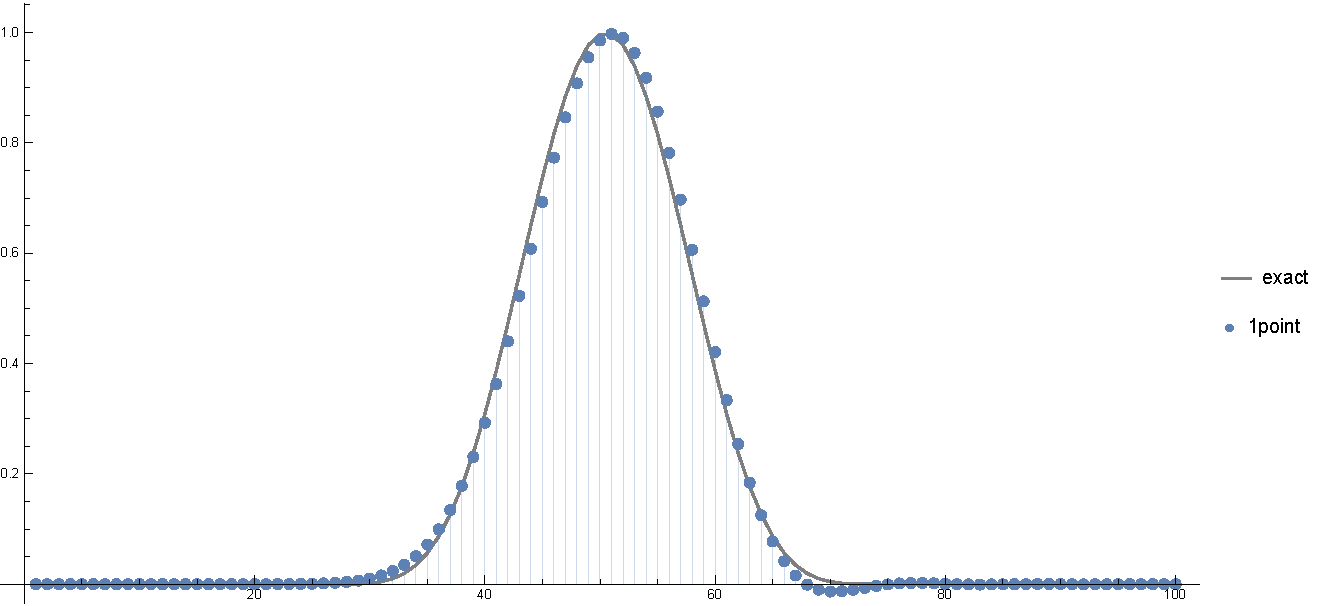
\includegraphics[width=\textwidth]{fig-1point-c0p8-T8-limit0-smooth.pdf}
	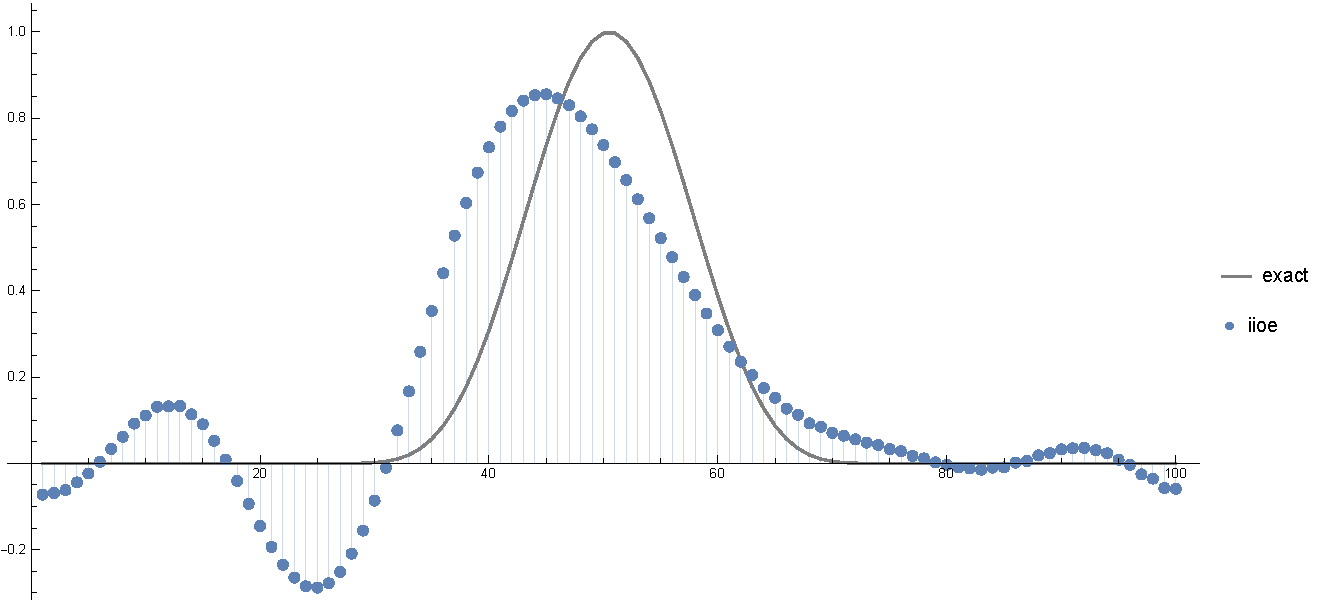
\includegraphics[width=\textwidth]{fig-iioe-c0p8-T8-limit0-smooth.pdf}
	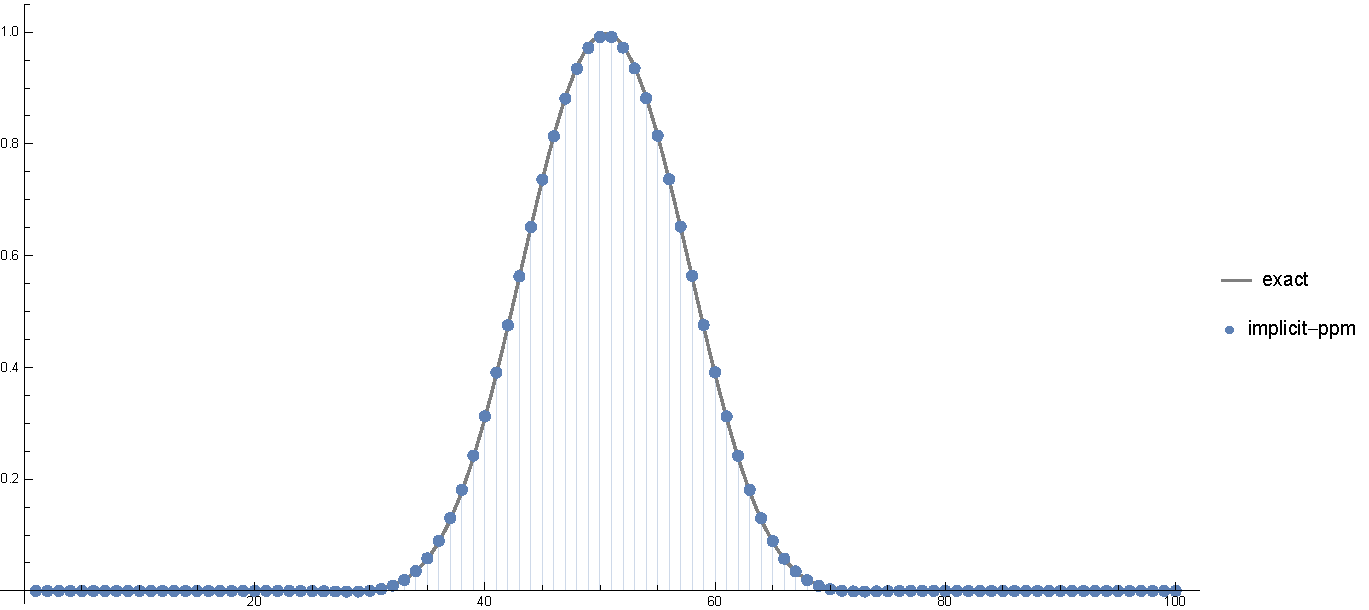
\includegraphics[width=\textwidth]{fig-implicit-ppm-c0p8-T8-limit0-smooth.pdf}
	\caption{Numerical solution after 4 cycles: second-order, implicit-upwind 1 point-scheme \eqref{eqn:1point-slope} (up), second-order, implicit, centered (IIOE) scheme \eqref{eqn:iioe-slope} (center), third-order, implicit, piecewise parabolic scheme \eqref{eqn:implicit-ppm-slope} (down). The Courant number is \(c = 0.8\), on a coarse grid with \(N = 100\) grid points, at time \(T = 8\), number of time steps 500.}
	\label{fig:c0p8-T8-limit0-smooth}
\end{figure}
\begin{figure}[H]
	\centering
    \caption*{Second-order, implicit-upwind 1 point-scheme \eqref{eqn:1point-slope}}
	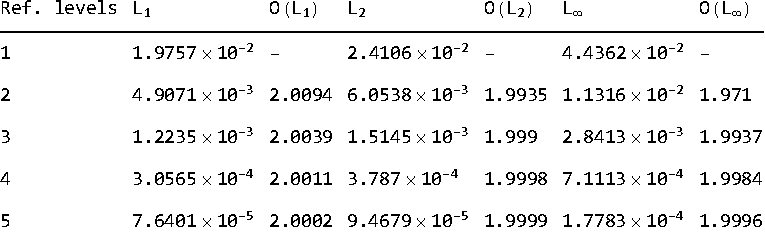
\includegraphics[width=\textwidth]{../tab/tab-1point-c0p8-T8-limit0-smooth.pdf}
    \caption*{second-order, implicit, centered (IIOE) scheme \eqref{eqn:iioe-slope}}
	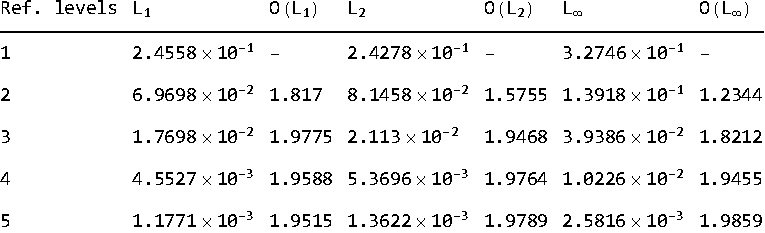
\includegraphics[width=\textwidth]{../tab/tab-iioe-c0p8-T8-limit0-smooth.pdf}
    \caption*{third-order, implicit, piecewise parabolic scheme \eqref{eqn:implicit-ppm-slope}}
	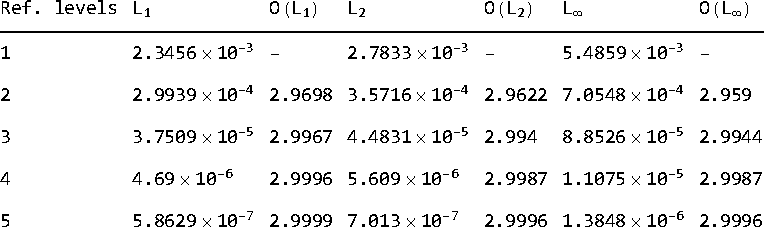
\includegraphics[width=\textwidth]{../tab/tab-implicit-ppm-c0p8-T8-limit0-smooth.pdf}
	\caption{Errors and experimental order of convergence of the numerical solution after 4 cycles: second-order, implicit-upwind 1 point-scheme \eqref{eqn:1point-slope} (up), second-order, implicit, centered (IIOE) scheme \eqref{eqn:iioe-slope} (center), third-order, implicit, piecewise parabolic scheme \eqref{eqn:implicit-ppm-slope} (down). The Courant number is \(c = 0.8\), on a coarse grid with \(N = 100\) grid points, at time \(T = 8\), number of time steps 500.}
	\label{tab:c0p8-T8-limit0-smooth}
\end{figure}
\begin{figure}[H]
	\centering
	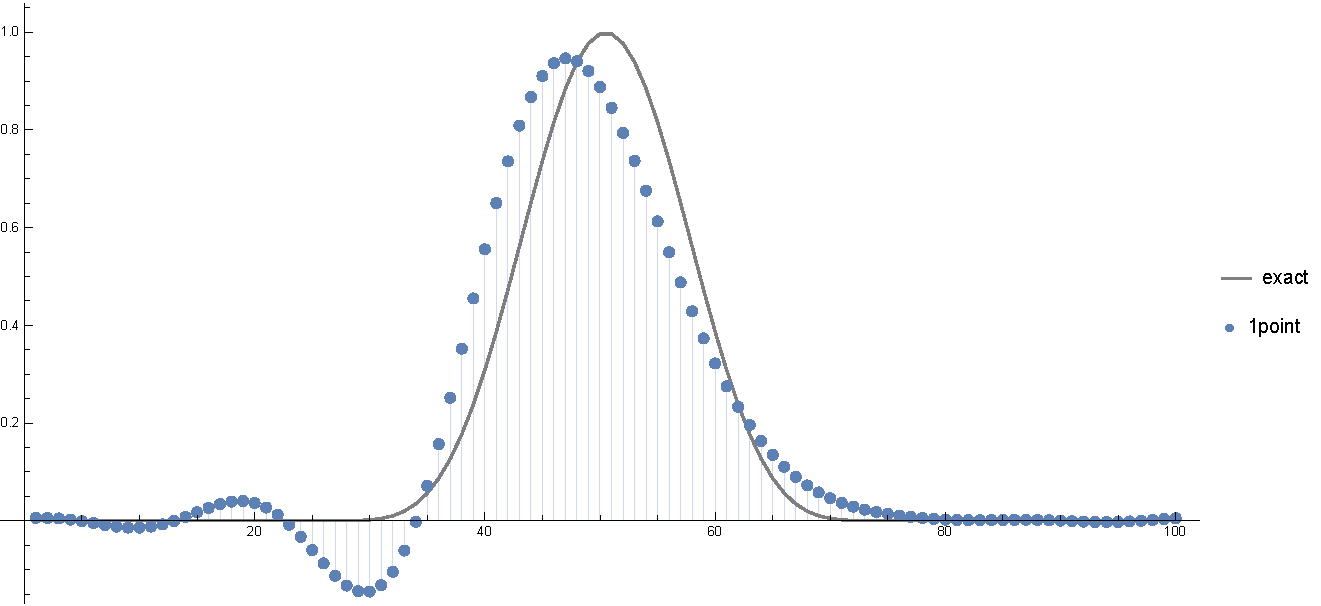
\includegraphics[width=\textwidth]{fig-1point-c1p8-T8-limit0-smooth.pdf}
	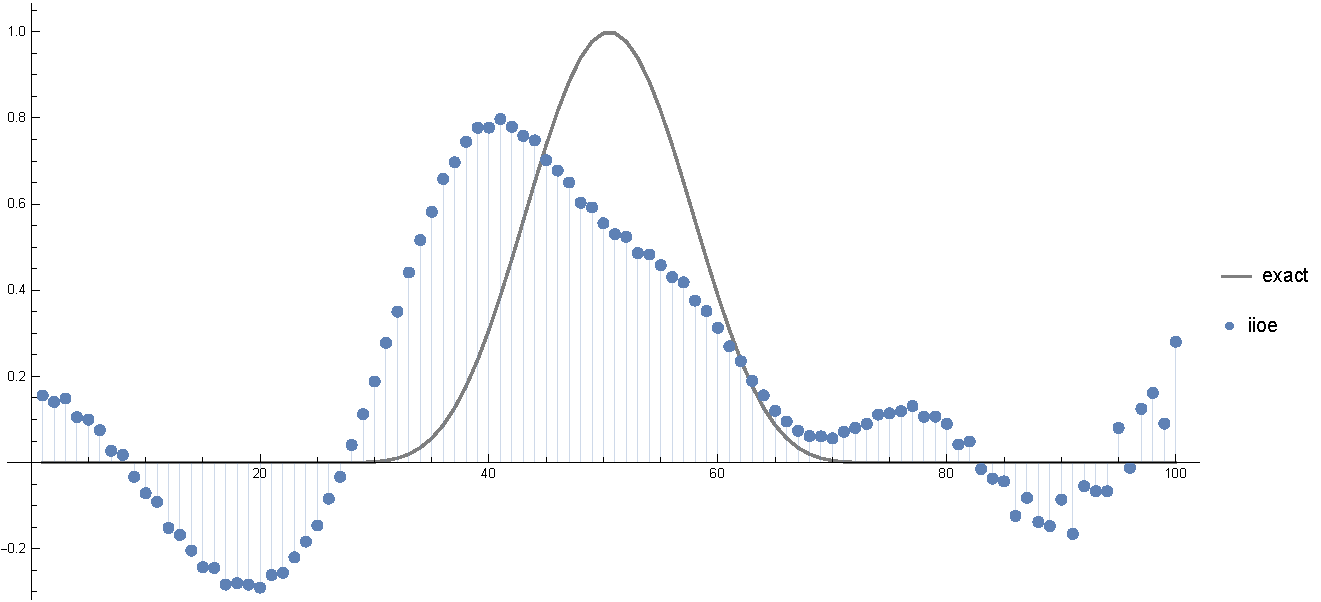
\includegraphics[width=\textwidth]{fig-iioe-c1p8-T8-limit0-smooth.pdf}
	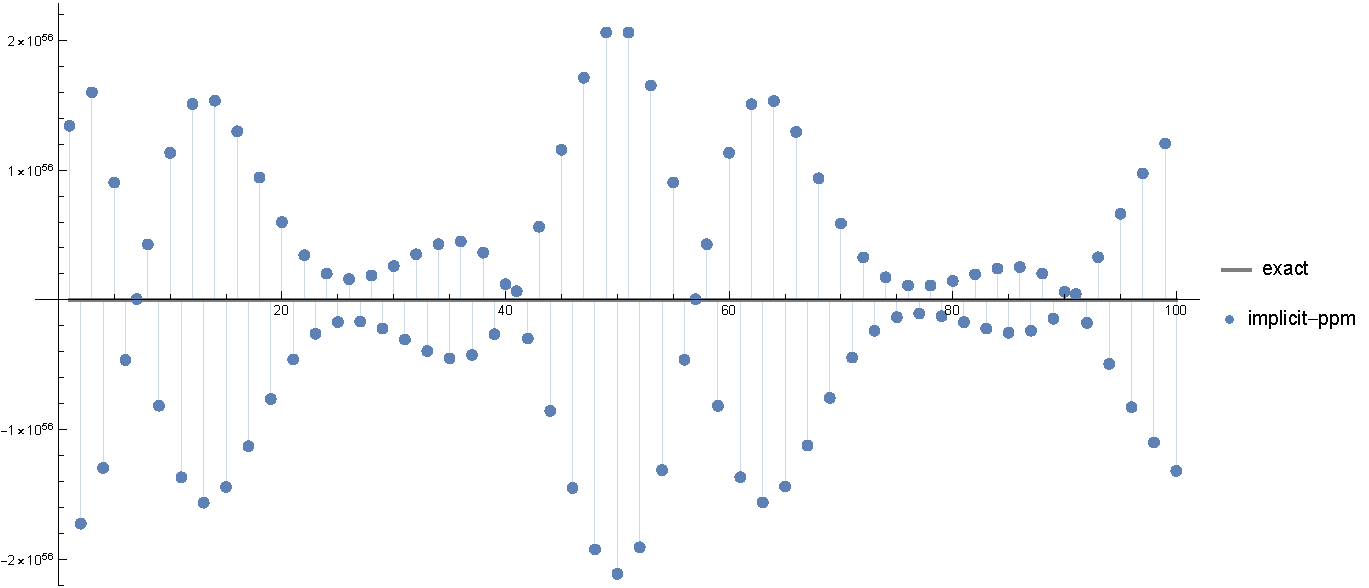
\includegraphics[width=\textwidth]{fig-implicit-ppm-c1p8-T8-limit0-smooth.pdf}
	\caption{Numerical solution after 4 cycles: second-order, implicit-upwind 1 point-scheme \eqref{eqn:1point-slope} (up), second-order, implicit, centered (IIOE) scheme \eqref{eqn:iioe-slope} (center), third-order, implicit, piecewise parabolic scheme \eqref{eqn:implicit-ppm-slope} (down). The Courant number is \(c = 1.8\), on a coarse grid with \(N = 100\) grid points, at time \(T = 8\), number of time steps 223.}
	\label{fig:c1p8-T8-limit0-smooth}
\end{figure}
\begin{figure}[H]
	\centering
    \caption*{Second-order, implicit-upwind 1 point-scheme \eqref{eqn:1point-slope}}
	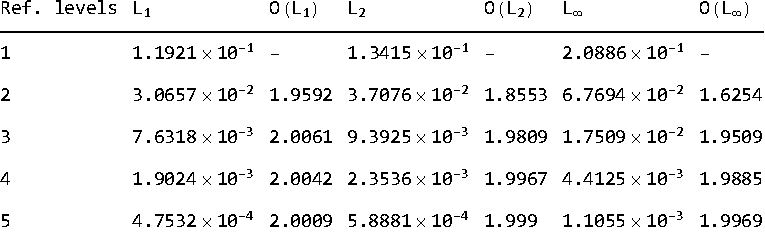
\includegraphics[width=\textwidth]{tab-1point-c1p8-T8-limit0-smooth.pdf}
    \caption*{second-order, implicit, centered (IIOE) scheme \eqref{eqn:iioe-slope}}
	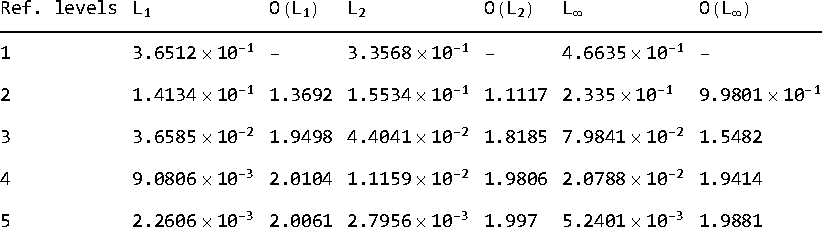
\includegraphics[width=\textwidth]{tab-iioe-c1p8-T8-limit0-smooth.pdf}
    \caption*{third-order, implicit, piecewise parabolic scheme \eqref{eqn:implicit-ppm-slope}}
	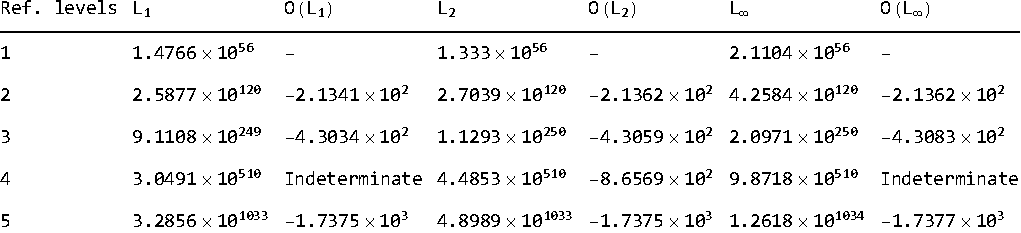
\includegraphics[width=\textwidth]{tab-implicit-ppm-c1p8-T8-limit0-smooth.pdf}
	\caption{Errors and experimental order of convergence of the numerical solution after 4 cycles: second-order, implicit-upwind 1 point-scheme \eqref{eqn:1point-slope} (up), second-order, implicit, centered (IIOE) scheme \eqref{eqn:iioe-slope} (center), third-order, implicit, piecewise parabolic scheme \eqref{eqn:implicit-ppm-slope} (down). The Courant number is \(c = 1.8\), on a coarse grid with \(N = 100\) grid points, at time \(T = 8\), number of time steps 223.}
	\label{tab:c1p8-T8-limit0-smooth}
\end{figure}
\subsubsection{Linear advection - smooth profile - limited}
\begin{figure}[H]
	\centering
	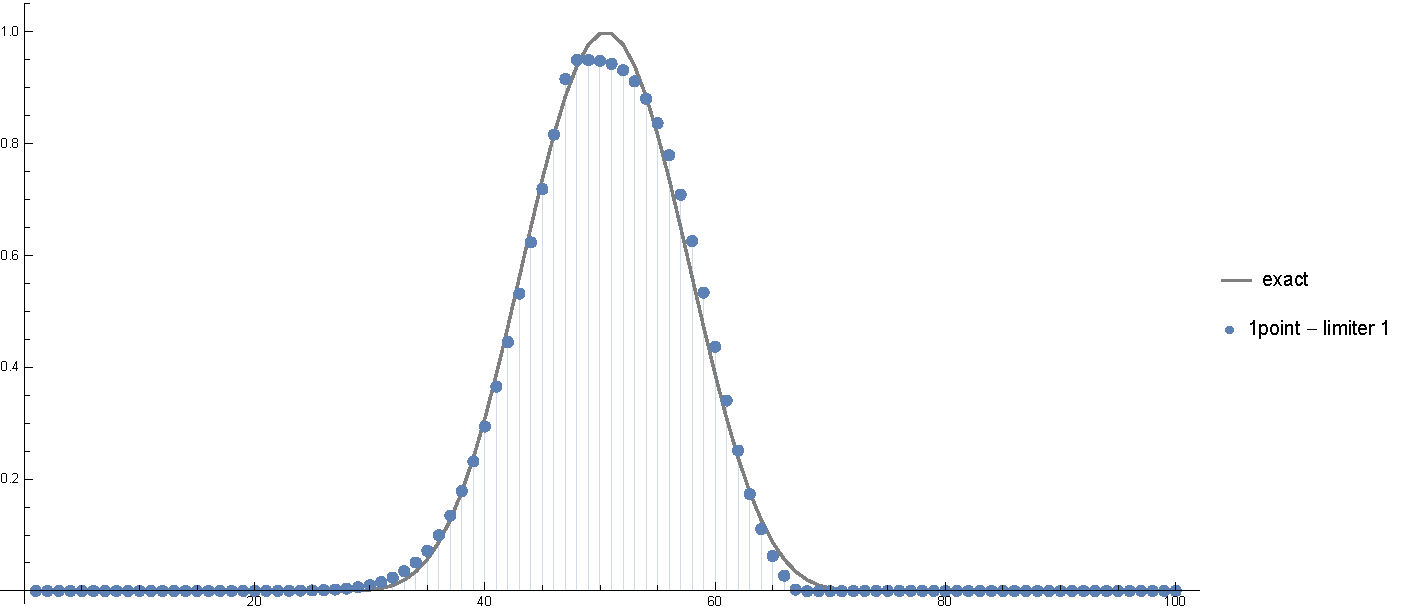
\includegraphics[width=\textwidth]{fig-1point-c0p8-T8-limit1-smooth.pdf}
	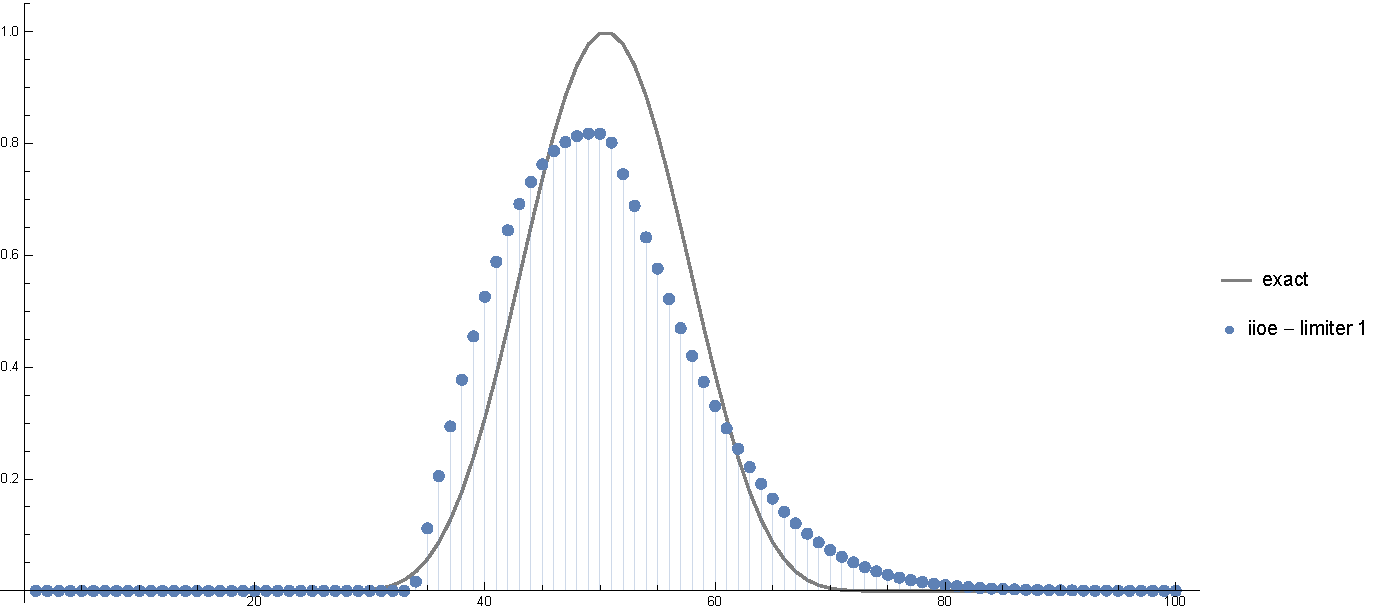
\includegraphics[width=\textwidth]{fig-iioe-c0p8-T8-limit1-smooth.pdf}
	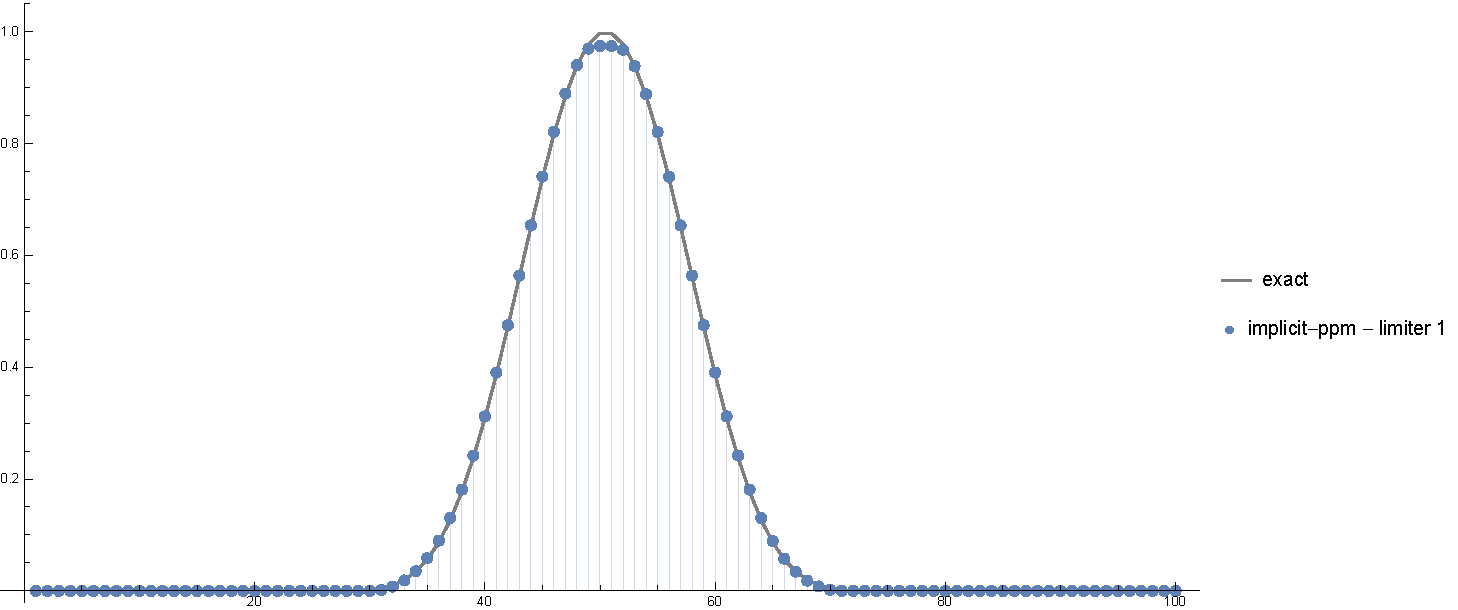
\includegraphics[width=\textwidth]{fig-implicit-ppm-c0p8-T8-limit1-smooth.pdf}
	\caption{Numerical solution after 4 cycles: second-order, implicit-upwind 1 point-scheme \eqref{eqn:1point-slope} (up), second-order, implicit, centered (IIOE) scheme \eqref{eqn:iioe-slope} (center), third-order, implicit, piecewise parabolic scheme \eqref{eqn:implicit-ppm-slope} (down). The Courant number is \(c = 0.8\), on a coarse grid with \(N = 100\) grid points, at time \(T = 8\), number of time steps 500.}
	\label{fig:c0p8-T8-limit1-smooth}
\end{figure}
\begin{figure}[H]
	\centering
    \caption*{Second-order, implicit-upwind 1 point-scheme \eqref{eqn:1point-slope} - limiter 1 \eqref{eqn:monotone-slope}}
	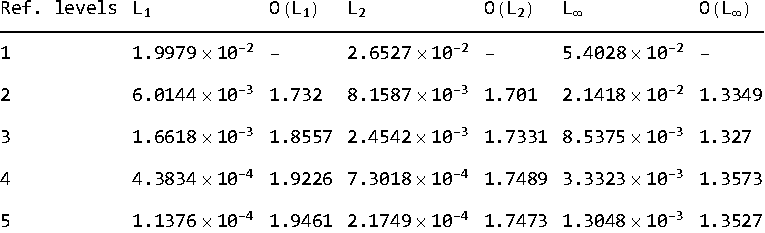
\includegraphics[width=\textwidth]{../tab/tab-1point-c0p8-T8-limit1-smooth.pdf}
    \caption*{second-order, implicit, centered (IIOE) scheme \eqref{eqn:iioe-slope} - limiter 1 \eqref{eqn:monotone-slope}}
	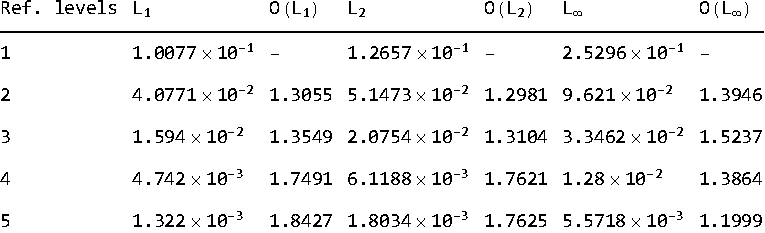
\includegraphics[width=\textwidth]{../tab/tab-iioe-c0p8-T8-limit1-smooth.pdf}
    \caption*{third-order, implicit, piecewise parabolic scheme \eqref{eqn:implicit-ppm-slope} - limiter 1 \eqref{eqn:monotone-slope}}
	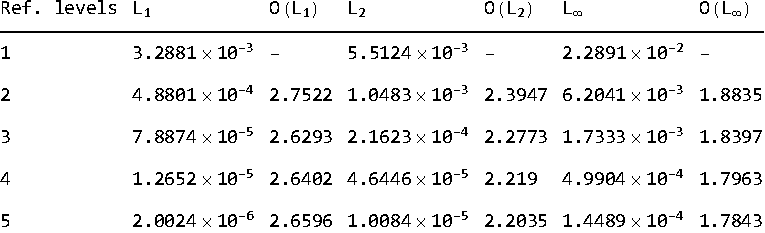
\includegraphics[width=\textwidth]{../tab/tab-implicit-ppm-c0p8-T8-limit1-smooth.pdf}
	\caption{Errors and experimental order of convergence of the numerical solution after 4 cycles: second-order, implicit-upwind 1 point-scheme \eqref{eqn:1point-slope} (up), second-order, implicit, centered (IIOE) scheme \eqref{eqn:iioe-slope} (center), third-order, implicit, piecewise parabolic scheme \eqref{eqn:implicit-ppm-slope} (down). The Courant number is \(c = 0.8\), on a coarse grid with \(N = 100\) grid points, at time \(T = 8\), number of time steps 500.}
	\label{tab:c0p8-T8-limit1-smooth}
\end{figure}
\begin{figure}[H]
	\centering
	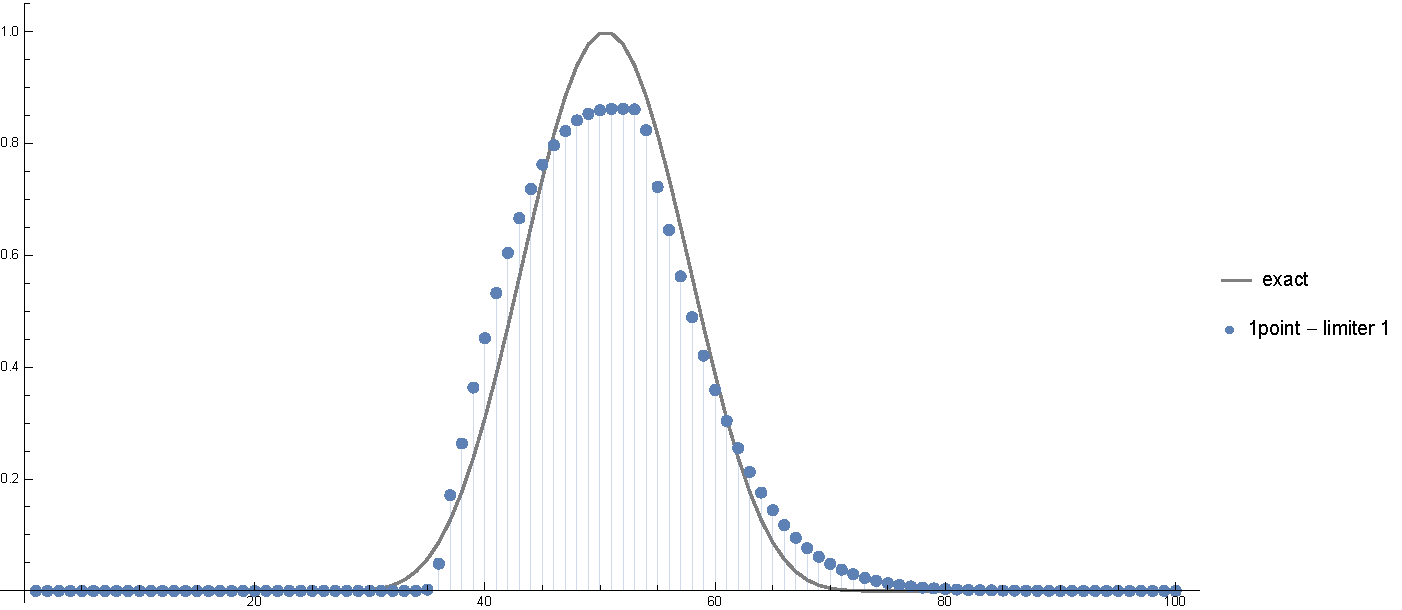
\includegraphics[width=\textwidth]{fig-1point-c1p8-T8-limit1-smooth.pdf}
	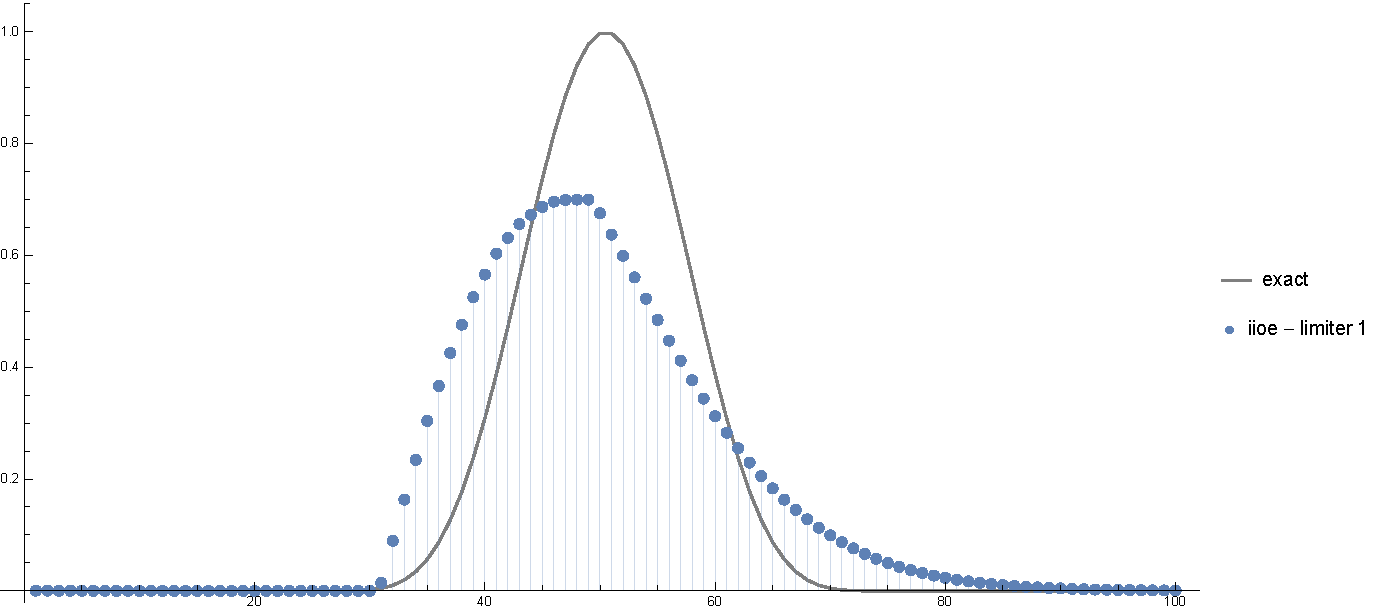
\includegraphics[width=\textwidth]{fig-iioe-c1p8-T8-limit1-smooth.pdf}
	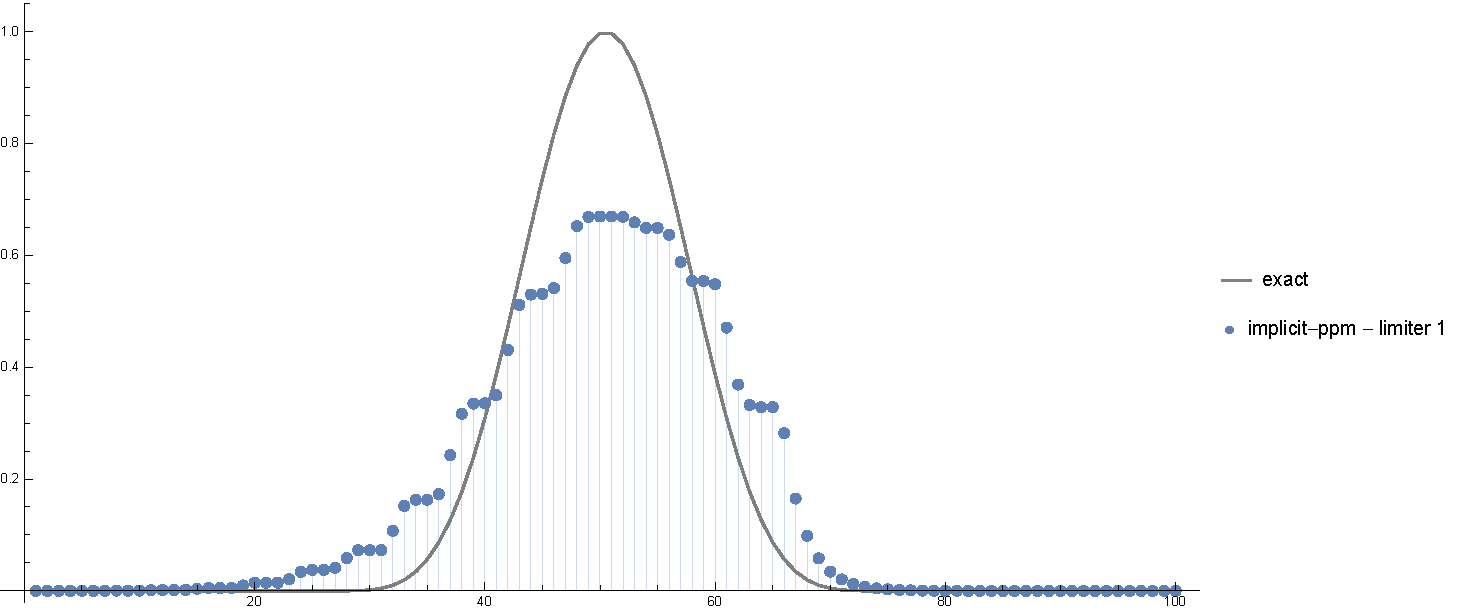
\includegraphics[width=\textwidth]{fig-implicit-ppm-c1p8-T8-limit1-smooth.pdf}
	\caption{Numerical solution after 4 cycles: second-order, implicit-upwind 1 point-scheme \eqref{eqn:1point-slope} (up), second-order, implicit, centered (IIOE) scheme \eqref{eqn:iioe-slope} (center), third-order, implicit, piecewise parabolic scheme \eqref{eqn:implicit-ppm-slope} (down). The Courant number is \(c = 1.8\), on a coarse grid with \(N = 100\) grid points, at time \(T = 8\), number of time steps 223.}
	\label{fig:c1p8-T8-limit1-smooth}
\end{figure}
\begin{figure}[H]
	\centering
    \caption*{Second-order, implicit-upwind 1 point-scheme \eqref{eqn:1point-slope} - limiter 1 \eqref{eqn:monotone-slope}}
	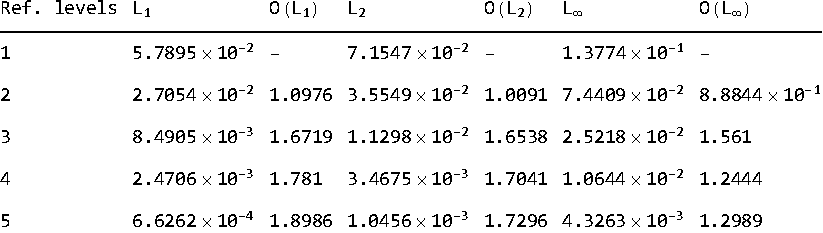
\includegraphics[width=\textwidth]{../tab/tab-1point-c1p8-T8-limit1-smooth.pdf}
    \caption*{second-order, implicit, centered (IIOE) scheme \eqref{eqn:iioe-slope} - limiter 1 \eqref{eqn:monotone-slope}}
	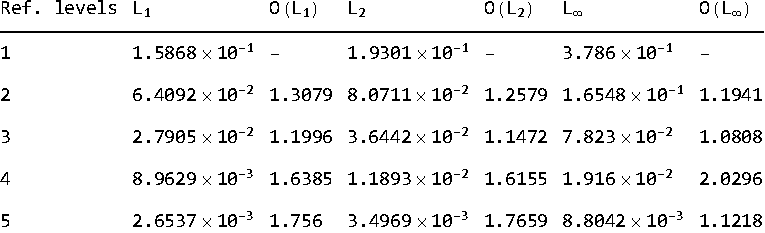
\includegraphics[width=\textwidth]{../tab/tab-iioe-c1p8-T8-limit1-smooth.pdf}
    \caption*{third-order, implicit, piecewise parabolic scheme \eqref{eqn:implicit-ppm-slope} - limiter 1 \eqref{eqn:monotone-slope}}
	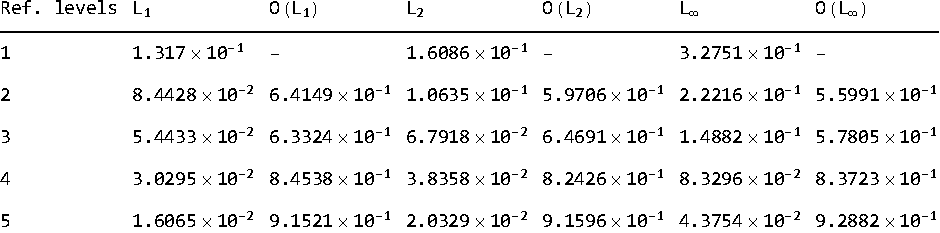
\includegraphics[width=\textwidth]{../tab/tab-implicit-ppm-c1p8-T8-limit1-smooth.pdf}
	\caption{Errors and experimental order of convergence of the numerical solution after 4 cycles: second-order, implicit-upwind 1 point-scheme \eqref{eqn:1point-slope} (up), second-order, implicit, centered (IIOE) scheme \eqref{eqn:iioe-slope} (center), third-order, implicit, piecewise parabolic scheme \eqref{eqn:implicit-ppm-slope} (down). The Courant number is \(c = 1.8\), on a coarse grid with \(N = 100\) grid points, at time \(T = 8\), number of time steps 223.}
	\label{tab:c1p8-T8-limit1-smooth}
\end{figure}
\begin{figure}[H]
	\centering
	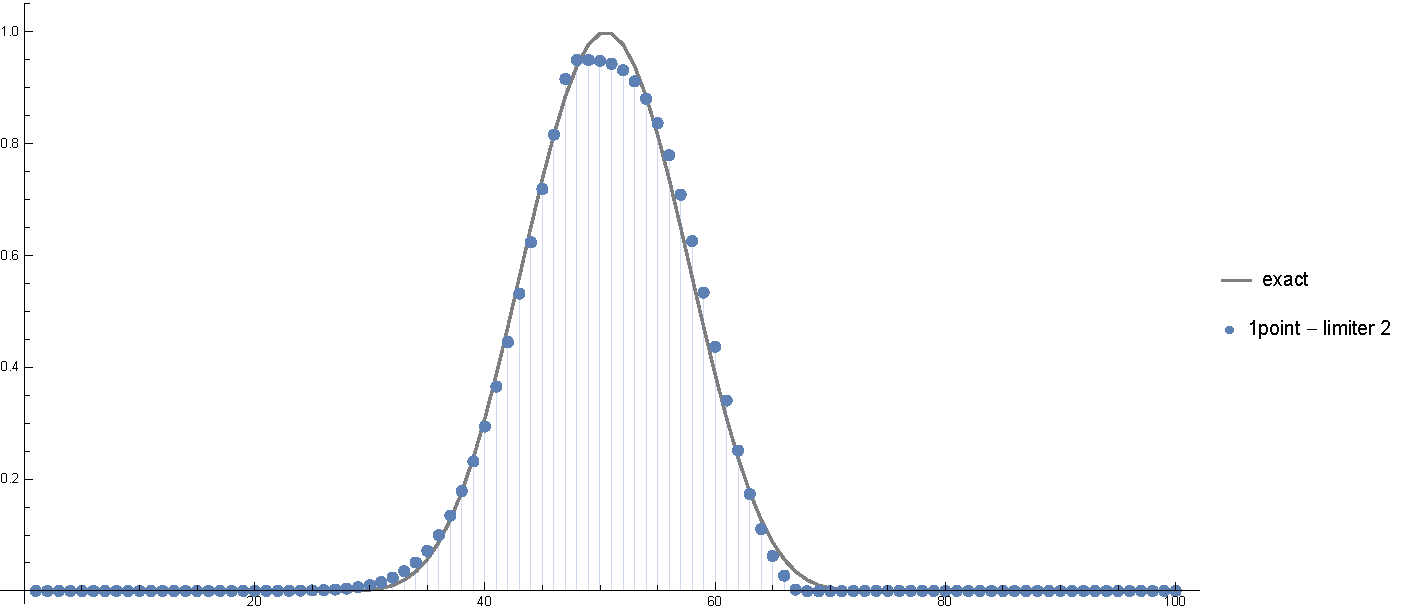
\includegraphics[width=\textwidth]{fig-1point-c0p8-T8-limit2-smooth.pdf}
	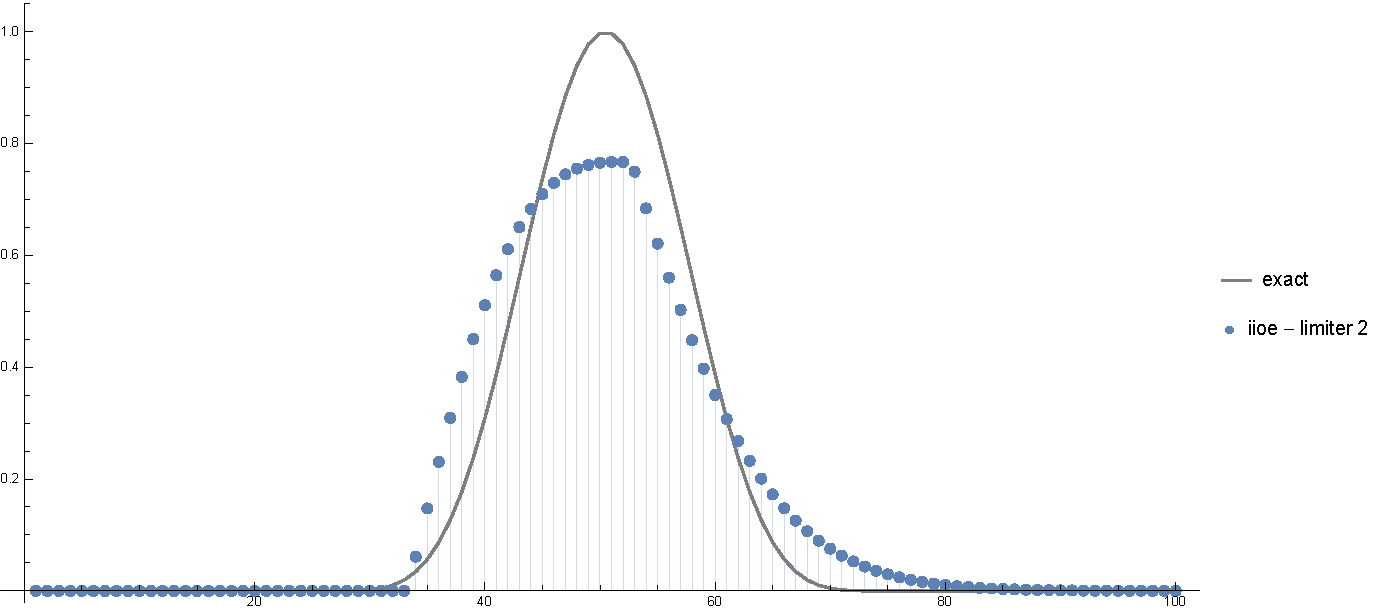
\includegraphics[width=\textwidth]{fig-iioe-c0p8-T8-limit2-smooth.pdf}
	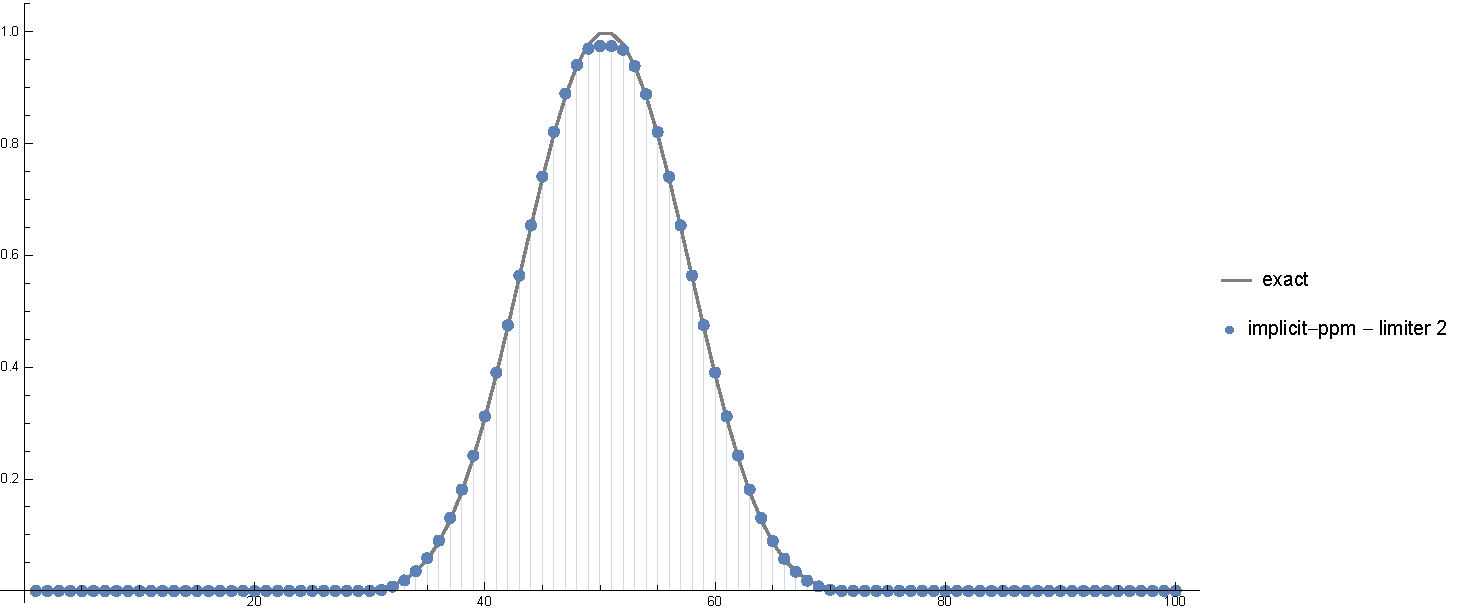
\includegraphics[width=\textwidth]{fig-implicit-ppm-c0p8-T8-limit2-smooth.pdf}
	\caption{Numerical solution after 4 cycles: second-order, implicit-upwind 1 point-scheme \eqref{eqn:1point-slope} (up), second-order, implicit, centered (IIOE) scheme \eqref{eqn:iioe-slope} (center), third-order, implicit, piecewise parabolic scheme \eqref{eqn:implicit-ppm-slope} (down). The Courant number is \(c = 0.8\), on a coarse grid with \(N = 100\) grid points, at time \(T = 8\), number of time steps 500.}
	\label{fig:c0p8-T8-limit2-smooth}
\end{figure}
\begin{figure}[H]
	\centering
    \caption*{Second-order, implicit-upwind 1 point-scheme \eqref{eqn:1point-slope} - limiter 2 \eqref{eqn:slope-sufficient}}
	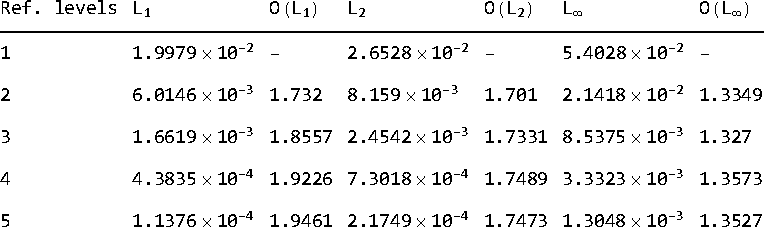
\includegraphics[width=\textwidth]{../tab/tab-1point-c0p8-T8-limit2-smooth.pdf}
    \caption*{second-order, implicit, centered (IIOE) scheme \eqref{eqn:iioe-slope} - limiter 2 \eqref{eqn:slope-sufficient}}
	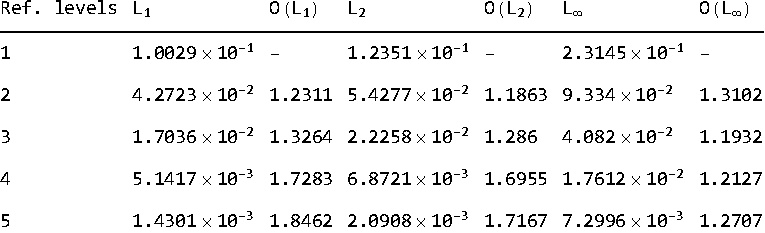
\includegraphics[width=\textwidth]{../tab/tab-iioe-c0p8-T8-limit2-smooth.pdf}
    \caption*{third-order, implicit, piecewise parabolic scheme \eqref{eqn:implicit-ppm-slope} - limiter 2 \eqref{eqn:slope-sufficient}}
	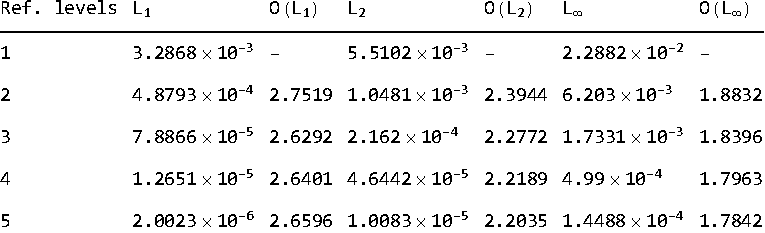
\includegraphics[width=\textwidth]{../tab/tab-implicit-ppm-c0p8-T8-limit2-smooth.pdf}
	\caption{Errors and experimental order of convergence of the numerical solution after 4 cycles: second-order, implicit-upwind 1 point-scheme \eqref{eqn:1point-slope} (up), second-order, implicit, centered (IIOE) scheme \eqref{eqn:iioe-slope} (center), third-order, implicit, piecewise parabolic scheme \eqref{eqn:implicit-ppm-slope} (down). The Courant number is \(c = 0.8\), on a coarse grid with \(N = 100\) grid points, at time \(T = 8\), number of time steps 500.}
	\label{tab:c0p8-T8-limit2-smooth}
\end{figure}
\begin{figure}[H]
	\centering
	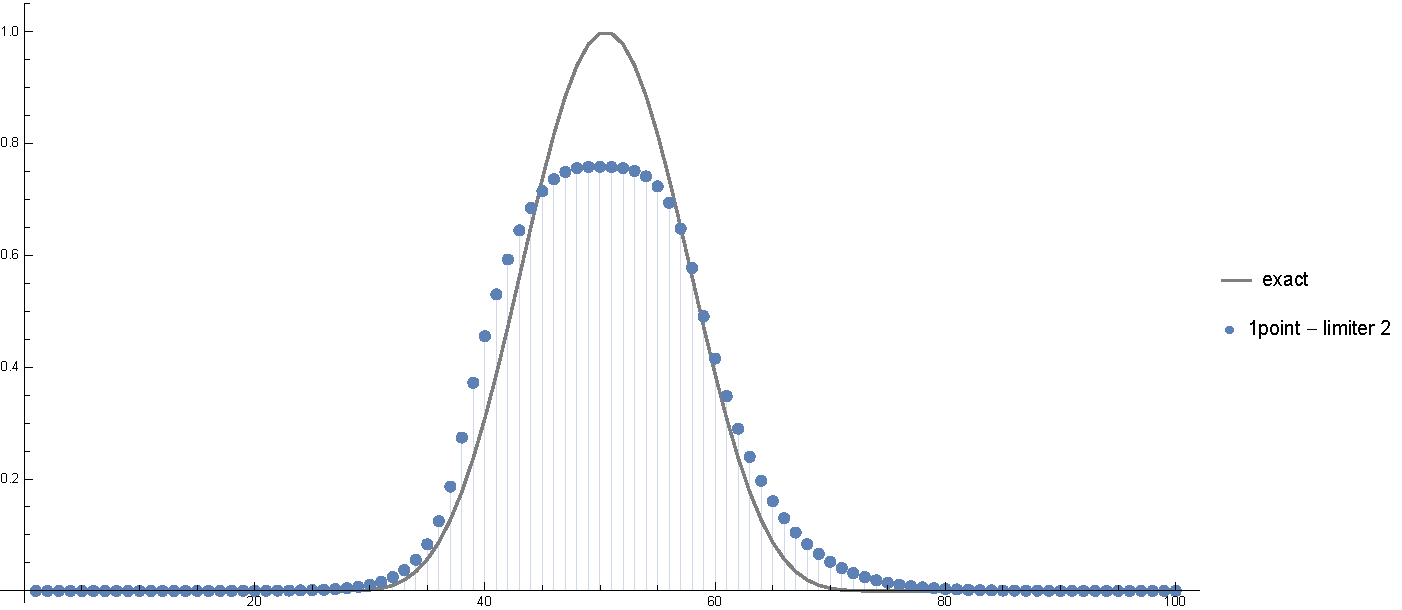
\includegraphics[width=\textwidth]{fig-1point-c1p8-T8-limit2-smooth.pdf}
	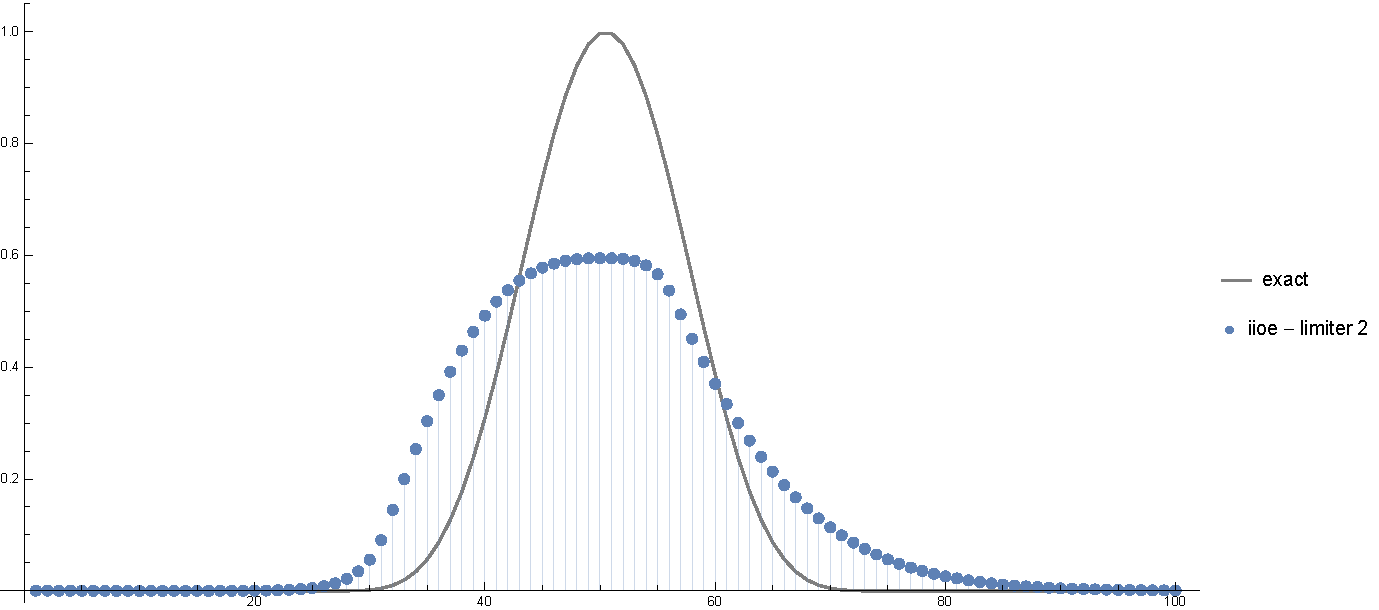
\includegraphics[width=\textwidth]{fig-iioe-c1p8-T8-limit2-smooth.pdf}
	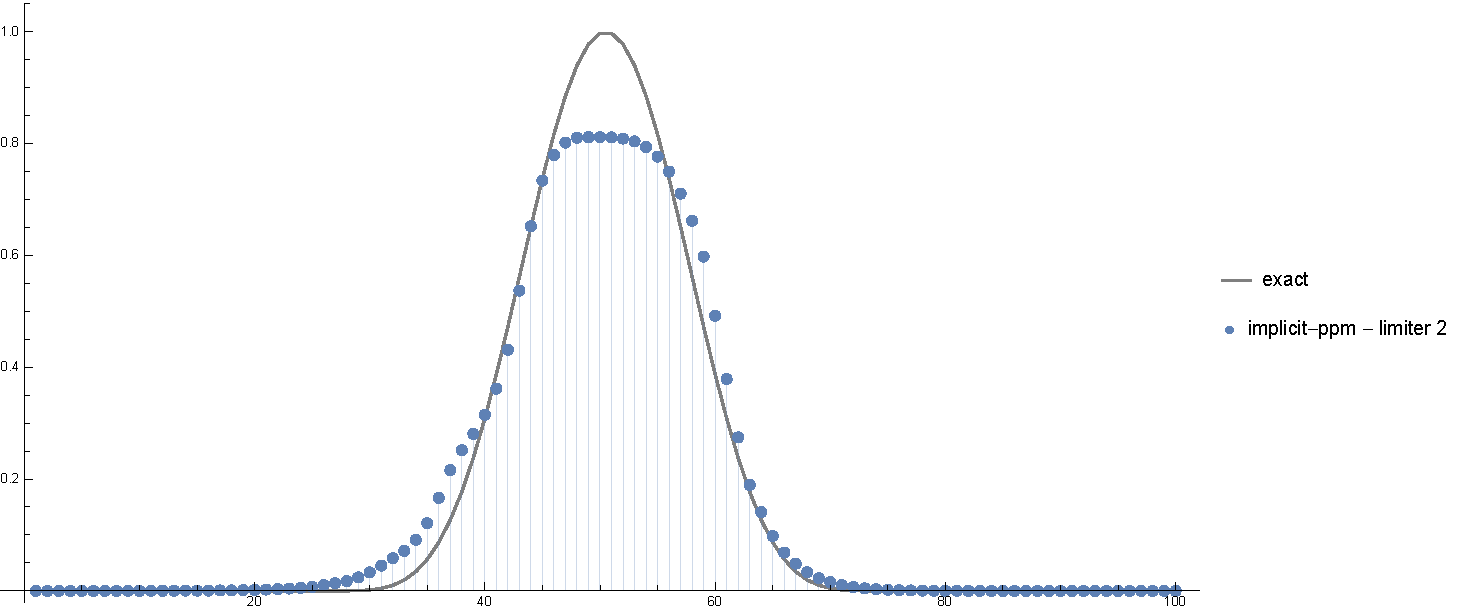
\includegraphics[width=\textwidth]{fig-implicit-ppm-c1p8-T8-limit2-smooth.pdf}
	\caption{Numerical solution after 4 cycles: second-order, implicit-upwind 1 point-scheme \eqref{eqn:1point-slope} (up), second-order, implicit, centered (IIOE) scheme \eqref{eqn:iioe-slope} (center), third-order, implicit, piecewise parabolic scheme \eqref{eqn:implicit-ppm-slope} (down). The Courant number is \(c = 1.8\), on a coarse grid with \(N = 100\) grid points, at time \(T = 8\), number of time steps 223.}
	\label{fig:c1p8-T8-limit2-smooth}
\end{figure}
\begin{figure}[H]
	\centering
    \caption*{Second-order, implicit-upwind 1 point-scheme \eqref{eqn:1point-slope} - limiter 2 \eqref{eqn:slope-sufficient}}
	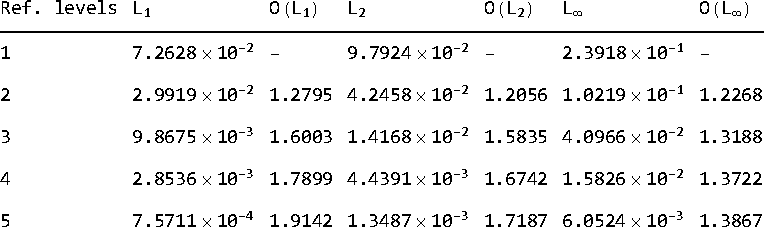
\includegraphics[width=\textwidth]{../tab/tab-1point-c1p8-T8-limit2-smooth.pdf}
    \caption*{second-order, implicit, centered (IIOE) scheme \eqref{eqn:iioe-slope} - limiter 2 \eqref{eqn:slope-sufficient}}
	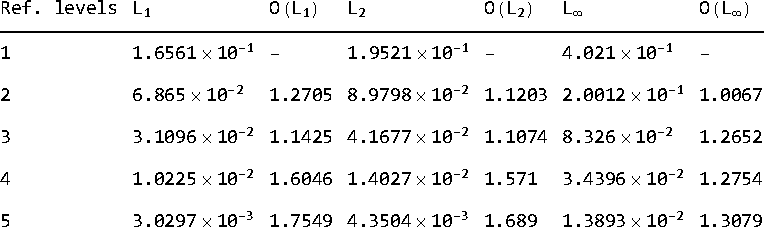
\includegraphics[width=\textwidth]{../tab/tab-iioe-c1p8-T8-limit2-smooth.pdf}
    \caption*{third-order, implicit, piecewise parabolic scheme \eqref{eqn:implicit-ppm-slope} - limiter 2 \eqref{eqn:slope-sufficient}}
	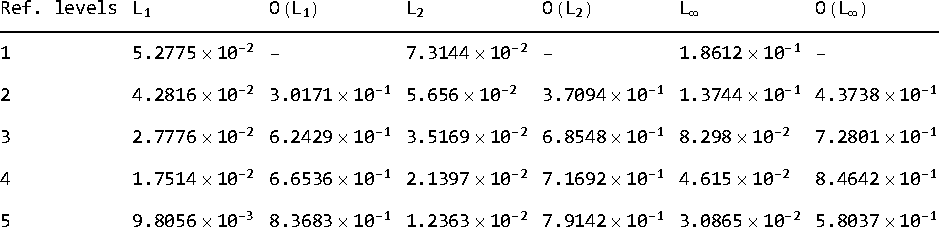
\includegraphics[width=\textwidth]{../tab/tab-implicit-ppm-c1p8-T8-limit2-smooth.pdf}
	\caption{Errors and experimental order of convergence of the numerical solution after 4 cycles: second-order, implicit-upwind 1 point-scheme \eqref{eqn:1point-slope} (up), second-order, implicit, centered (IIOE) scheme \eqref{eqn:iioe-slope} (center), third-order, implicit, piecewise parabolic scheme \eqref{eqn:implicit-ppm-slope} (down). The Courant number is \(c = 1.8\), on a coarse grid with \(N = 100\) grid points, at time \(T = 8\), number of time steps 223.}
	\label{tab:c1p8-T8-limit2-smooth}
\end{figure}
\subsubsection{Linear advection - discontinuities - unlimited}
\begin{figure}[H]
	\centering
	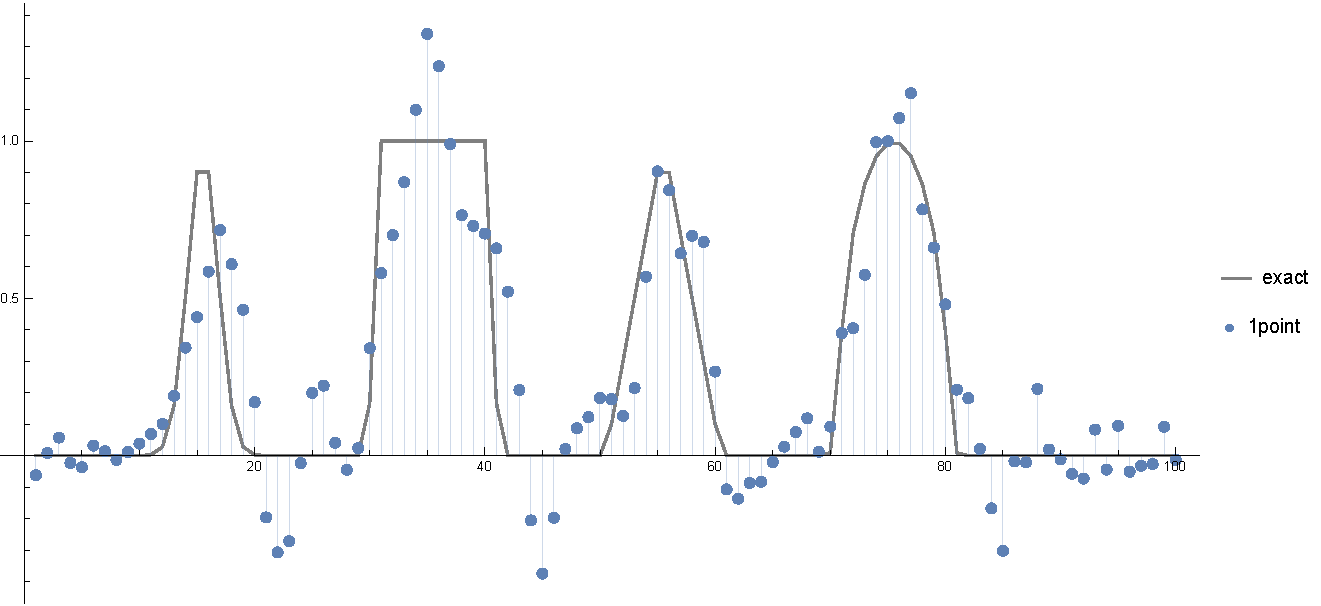
\includegraphics[width=\textwidth]{fig-1point-c0p8-T2-limit0-shu.pdf}
	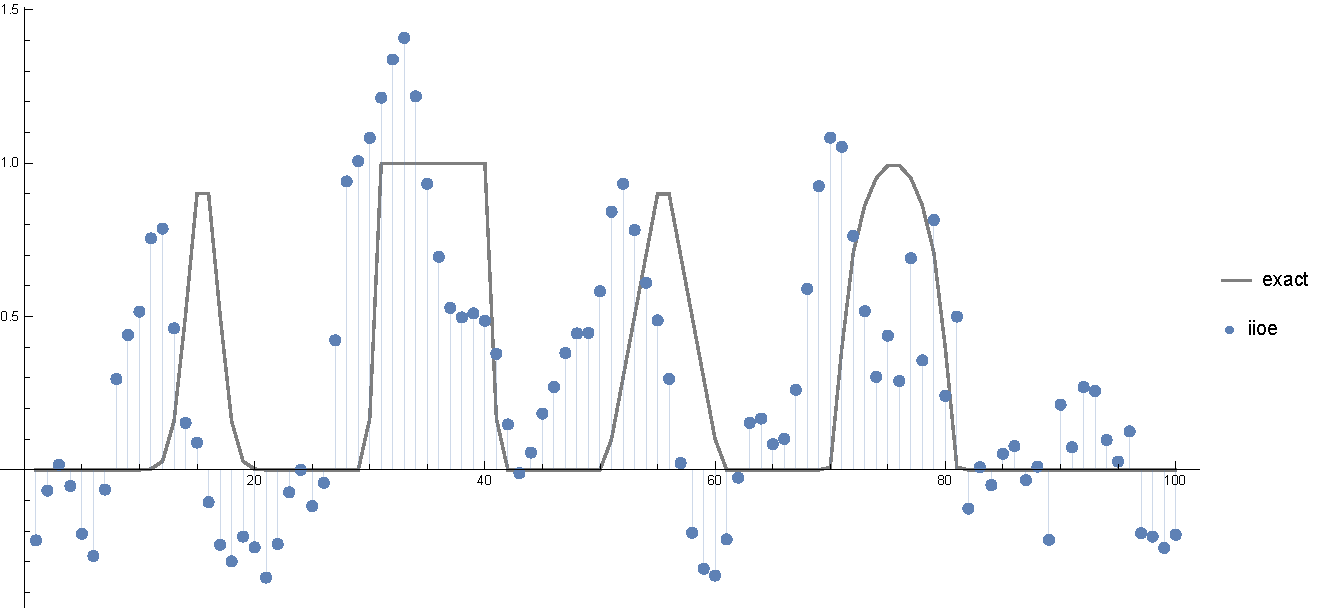
\includegraphics[width=\textwidth]{fig-iioe-c0p8-T2-limit0-shu.pdf}
	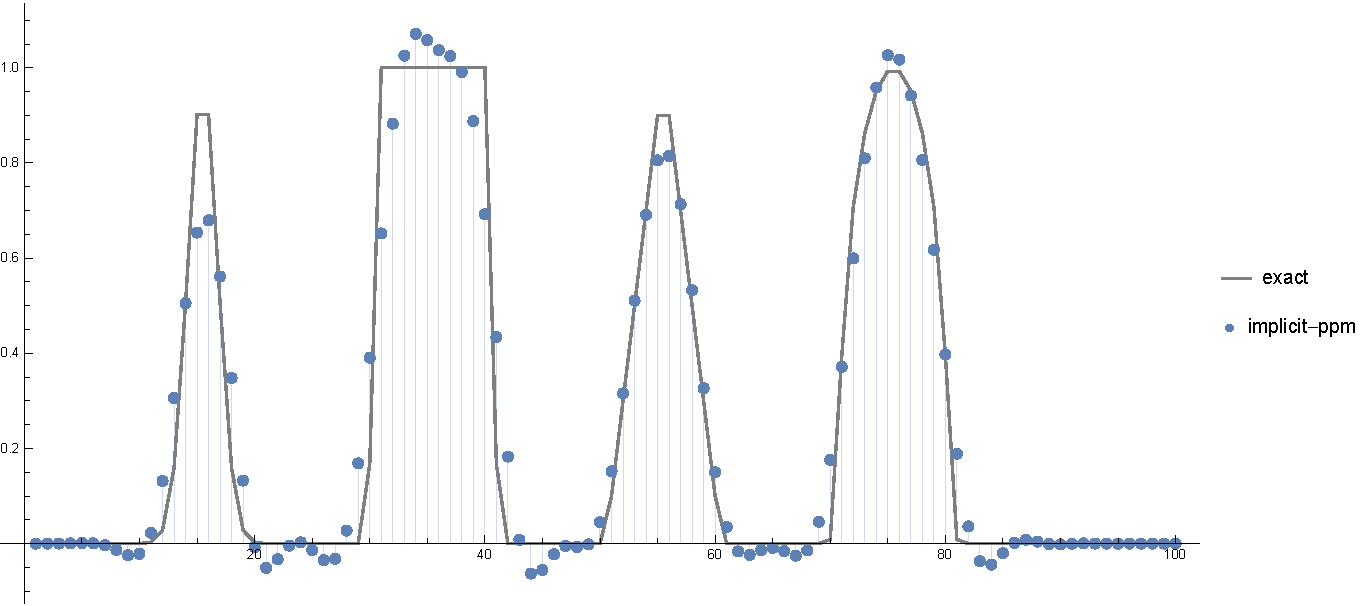
\includegraphics[width=\textwidth]{fig-implicit-ppm-c0p8-T2-limit0-shu.pdf}
	\caption{Numerical solution after 1 cycle: second-order, implicit-upwind 1 point-scheme \eqref{eqn:1point-slope} (up), second-order, implicit, centered (IIOE) scheme \eqref{eqn:iioe-slope} (center), third-order, implicit, piecewise parabolic scheme \eqref{eqn:implicit-ppm-slope} (down). The Courant number is \(c = 0.8\), on a coarse grid with \(N = 100\) grid points, at time \(T = 2\), number of time steps 125.}
	\label{fig:c0p8-T2-limit0-shu}
\end{figure}
\begin{figure}[H]
	\centering
    \caption*{Second-order, implicit-upwind 1 point-scheme \eqref{eqn:1point-slope}}
	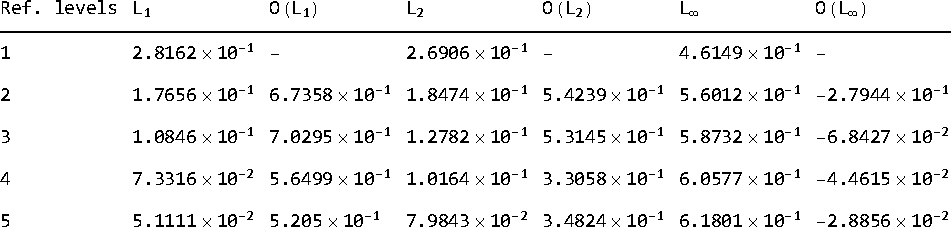
\includegraphics[width=\textwidth]{../tab/tab-1point-c0p8-T2-limit0-shu.pdf}
    \caption*{second-order, implicit, centered (IIOE) scheme \eqref{eqn:iioe-slope}}
	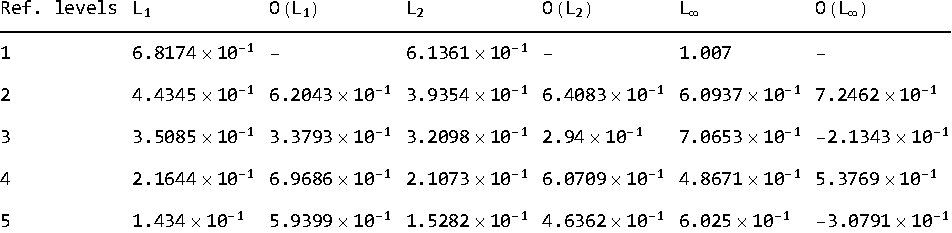
\includegraphics[width=\textwidth]{../tab/tab-iioe-c0p8-T2-limit0-shu.pdf}
    \caption*{third-order, implicit, piecewise parabolic scheme \eqref{eqn:implicit-ppm-slope}}
	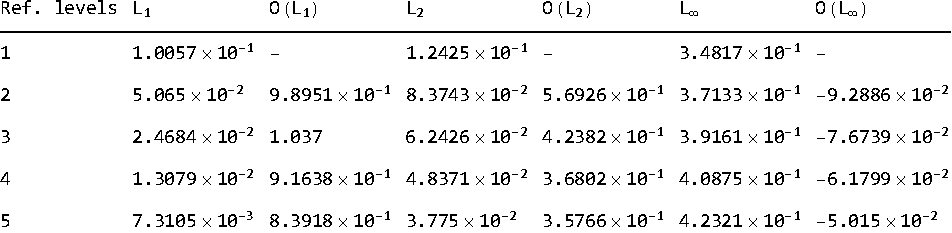
\includegraphics[width=\textwidth]{../tab/tab-implicit-ppm-c0p8-T2-limit0-shu.pdf}
	\caption{Errors and experimental order of convergence of the numerical solution after 1 cycle: second-order, implicit-upwind 1 point-scheme \eqref{eqn:1point-slope} (up), second-order, implicit, centered (IIOE) scheme \eqref{eqn:iioe-slope} (center), third-order, implicit, piecewise parabolic scheme \eqref{eqn:implicit-ppm-slope} (down). The Courant number is \(c = 0.8\), on a coarse grid with \(N = 100\) grid points, at time \(T = 2\), number of time steps 125.}
	\label{tab:c0p8-T2-limit0-shu}
\end{figure}
\begin{figure}[H]
	\centering
	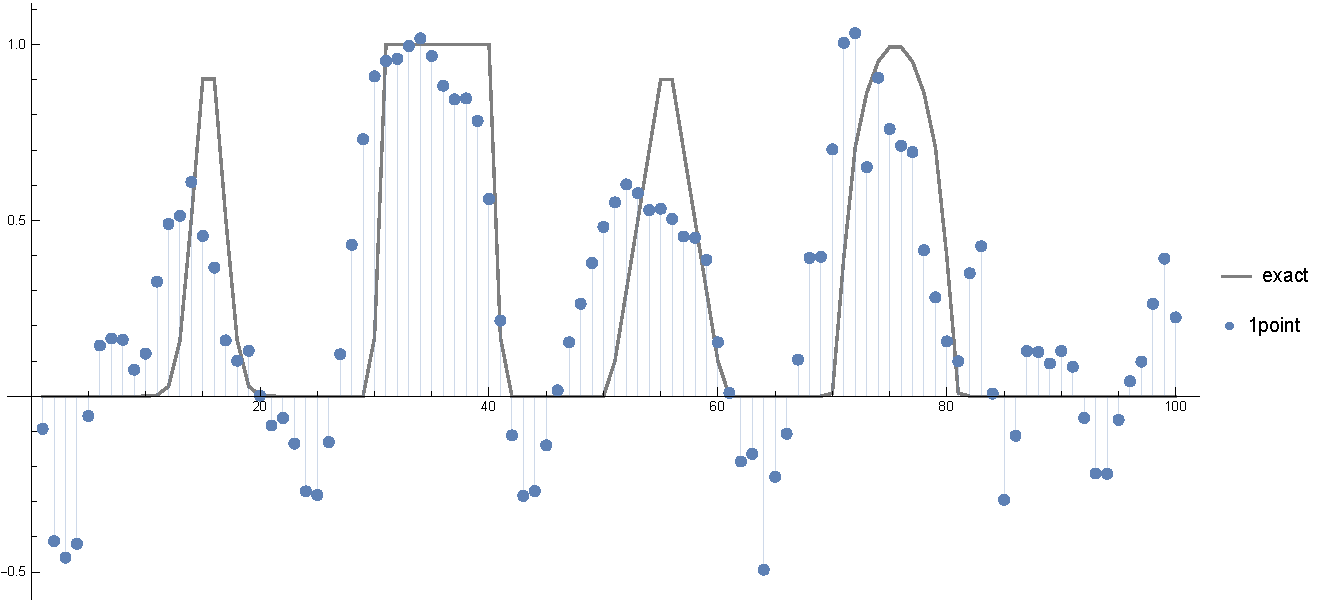
\includegraphics[width=\textwidth]{fig-1point-c1p8-T2-limit0-shu.pdf}
	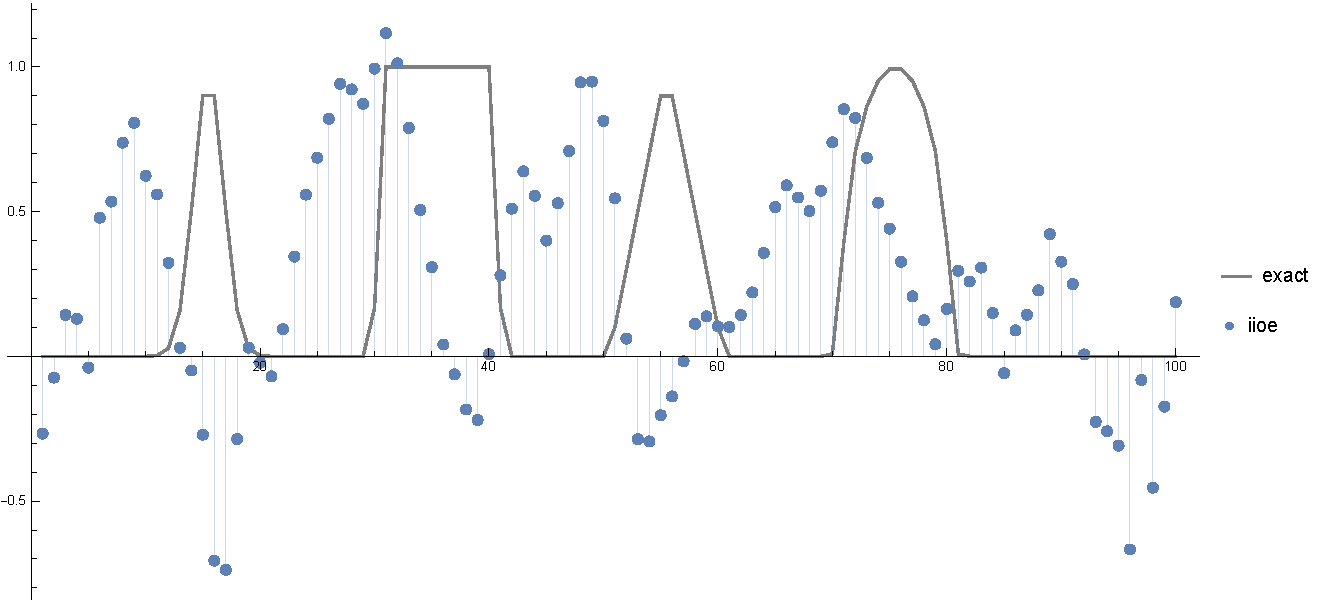
\includegraphics[width=\textwidth]{fig-iioe-c1p8-T2-limit0-shu.pdf}
	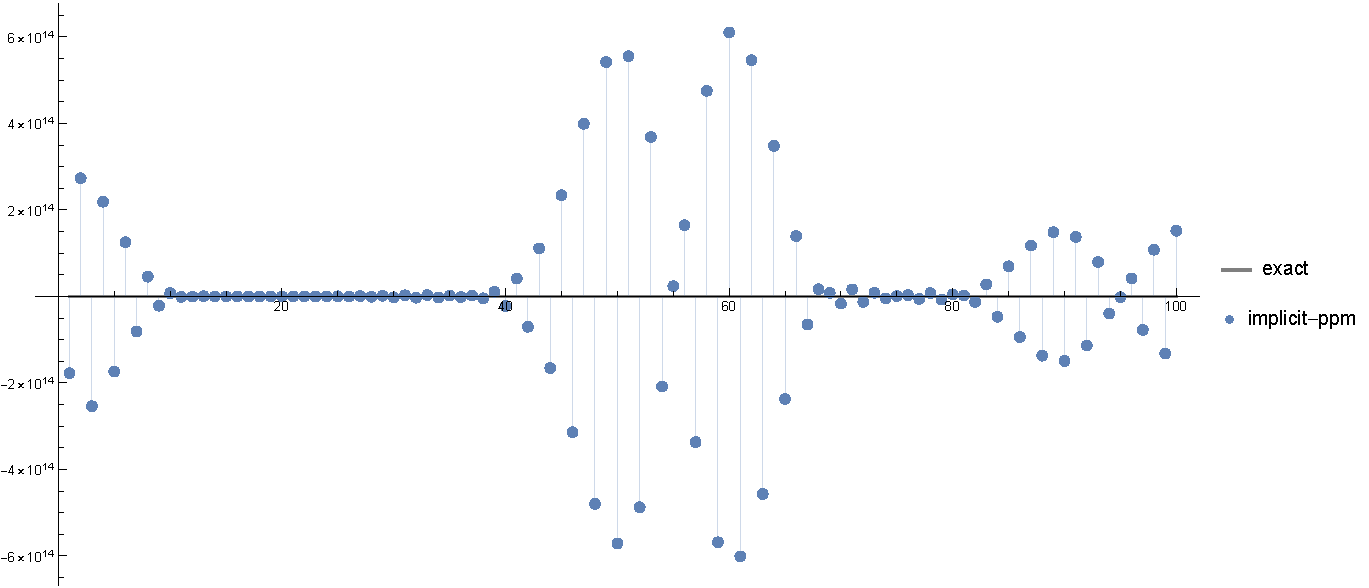
\includegraphics[width=\textwidth]{fig-implicit-ppm-c1p8-T2-limit0-shu.pdf}
	\caption{Numerical solution after 1 cycle: second-order, implicit-upwind 1 point-scheme \eqref{eqn:1point-slope} (up), second-order, implicit, centered (IIOE) scheme \eqref{eqn:iioe-slope} (center), third-order, implicit, piecewise parabolic scheme \eqref{eqn:implicit-ppm-slope} (down). The Courant number is \(c = 1.8\), on a coarse grid with \(N = 100\) grid points, at time \(T = 2\), number of time steps 56.}
	\label{fig:c1p8-T2-limit0-shu}
\end{figure}
\begin{figure}[H]
	\centering
    \caption*{Second-order, implicit-upwind 1 point-scheme \eqref{eqn:1point-slope}}
	\includegraphics[width=\textwidth]{../tab/tab-1point-c1p8-T2-limit0-shu.pdf}
    \caption*{second-order, implicit, centered (IIOE) scheme \eqref{eqn:iioe-slope}}
	\includegraphics[width=\textwidth]{../tab/tab-iioe-c1p8-T2-limit0-shu.pdf}
    \caption*{third-order, implicit, piecewise parabolic scheme \eqref{eqn:implicit-ppm-slope}}
	\includegraphics[width=\textwidth]{../tab/tab-implicit-ppm-c1p8-T2-limit0-shu.pdf}
	\caption{Errors and experimental order of convergence of the numerical solution after 1 cycle: second-order, implicit-upwind 1 point-scheme \eqref{eqn:1point-slope} (up), second-order, implicit, centered (IIOE) scheme \eqref{eqn:iioe-slope} (center), third-order, implicit, piecewise parabolic scheme \eqref{eqn:implicit-ppm-slope} (down). The Courant number is \(c = 1.8\), on a coarse grid with \(N = 100\) grid points, at time \(T = 2\), number of time steps 56.}
	\label{tab:c1p8-T2-limit0-shu}
\end{figure}
\subsubsection{Linear advection - discontinuities - limited}
\begin{figure}[H]
	\centering
	\includegraphics[width=\textwidth]{fig-1point-c0p8-T2-limit1-shu.pdf}
	\includegraphics[width=\textwidth]{fig-iioe-c0p8-T2-limit1-shu.pdf}
	\includegraphics[width=\textwidth]{fig-implicit-ppm-c0p8-T2-limit1-shu.pdf}
	\caption{Numerical solution after 1 cycle: second-order, implicit-upwind 1 point-scheme \eqref{eqn:1point-slope} (up), second-order, implicit, centered (IIOE) scheme \eqref{eqn:iioe-slope} (center), third-order, implicit, piecewise parabolic scheme \eqref{eqn:implicit-ppm-slope} (down). The Courant number is \(c = 0.8\), on a coarse grid with \(N = 100\) grid points, at time \(T = 2\), number of time steps 125.}
	\label{fig:c0p8-T2-limit1-shu}
\end{figure}
\begin{figure}[H]
	\centering
    \caption*{Second-order, implicit-upwind 1 point-scheme \eqref{eqn:1point-slope} - limiter 1 \eqref{eqn:monotone-slope}}
	\includegraphics[width=\textwidth]{../tab/tab-1point-c0p8-T2-limit1-shu.pdf}
    \caption*{second-order, implicit, centered (IIOE) scheme \eqref{eqn:iioe-slope} - limiter 1 \eqref{eqn:monotone-slope}}
	\includegraphics[width=\textwidth]{../tab/tab-iioe-c0p8-T2-limit1-shu.pdf}
    \caption*{third-order, implicit, piecewise parabolic scheme \eqref{eqn:implicit-ppm-slope} - limiter 1 \eqref{eqn:monotone-slope}}
	\includegraphics[width=\textwidth]{../tab/tab-implicit-ppm-c0p8-T2-limit1-shu.pdf}
	\caption{Errors and experimental order of convergence of the numerical solution after 1 cycle: second-order, implicit-upwind 1 point-scheme \eqref{eqn:1point-slope} (up), second-order, implicit, centered (IIOE) scheme \eqref{eqn:iioe-slope} (center), third-order, implicit, piecewise parabolic scheme \eqref{eqn:implicit-ppm-slope} (down). The Courant number is \(c = 0.8\), on a coarse grid with \(N = 100\) grid points, at time \(T = 2\), number of time steps 125.}
	\label{tab:c0p8-T2-limit1-shu}
\end{figure}
\begin{figure}[H]
	\centering
	\includegraphics[width=\textwidth]{fig-1point-c1p8-T2-limit1-shu.pdf}
	\includegraphics[width=\textwidth]{fig-iioe-c1p8-T2-limit1-shu.pdf}
	\includegraphics[width=\textwidth]{fig-implicit-ppm-c1p8-T2-limit1-shu.pdf}
	\caption{Numerical solution after 1 cycle: second-order, implicit-upwind 1 point-scheme \eqref{eqn:1point-slope} (up), second-order, implicit, centered (IIOE) scheme \eqref{eqn:iioe-slope} (center), third-order, implicit, piecewise parabolic scheme \eqref{eqn:implicit-ppm-slope} (down). The Courant number is \(c = 1.8\), on a coarse grid with \(N = 100\) grid points, at time \(T = 2\), number of time steps 56.}
	\label{fig:c1p8-T2-limit1-shu}
\end{figure}
\begin{figure}[H]
	\centering
    \caption*{Second-order, implicit-upwind 1 point-scheme \eqref{eqn:1point-slope} - limiter 1 \eqref{eqn:monotone-slope}}
	\includegraphics[width=\textwidth]{../tab/tab-1point-c1p8-T2-limit1-shu.pdf}
    \caption*{second-order, implicit, centered (IIOE) scheme \eqref{eqn:iioe-slope} - limiter 1 \eqref{eqn:monotone-slope}}
	\includegraphics[width=\textwidth]{../tab/tab-iioe-c1p8-T2-limit1-shu.pdf}
    \caption*{third-order, implicit, piecewise parabolic scheme \eqref{eqn:implicit-ppm-slope} - limiter 1 \eqref{eqn:monotone-slope}}
	\includegraphics[width=\textwidth]{../tab/tab-implicit-ppm-c1p8-T2-limit1-shu.pdf}
	\caption{Errors and experimental order of convergence of the numerical solution after 1 cycle: second-order, implicit-upwind 1 point-scheme \eqref{eqn:1point-slope} (up), second-order, implicit, centered (IIOE) scheme \eqref{eqn:iioe-slope} (center), third-order, implicit, piecewise parabolic scheme \eqref{eqn:implicit-ppm-slope} (down). The Courant number is \(c = 1.8\), on a coarse grid with \(N = 100\) grid points, at time \(T = 2\), number of time steps 56.}
	\label{tab:c1p8-T2-limit1-shu}
\end{figure}
\begin{figure}[H]
	\centering
	\includegraphics[width=\textwidth]{fig-1point-c0p8-T2-limit2-shu.pdf}
	\includegraphics[width=\textwidth]{fig-iioe-c0p8-T2-limit2-shu.pdf}
	\includegraphics[width=\textwidth]{fig-implicit-ppm-c0p8-T2-limit2-shu.pdf}
	\caption{Numerical solution after 1 cycle: second-order, implicit-upwind 1 point-scheme \eqref{eqn:1point-slope} (up), second-order, implicit, centered (IIOE) scheme \eqref{eqn:iioe-slope} (center), third-order, implicit, piecewise parabolic scheme \eqref{eqn:implicit-ppm-slope} (down). The Courant number is \(c = 0.8\), on a coarse grid with \(N = 100\) grid points, at time \(T = 2\), number of time steps 125.}
	\label{fig:c0p8-T2-limit2-shu}
\end{figure}
\begin{figure}[H]
	\centering
    \caption*{Second-order, implicit-upwind 1 point-scheme \eqref{eqn:1point-slope} - limiter 2 \eqref{eqn:slope-sufficient}}
	\includegraphics[width=\textwidth]{../tab/tab-1point-c0p8-T2-limit2-shu.pdf}
    \caption*{second-order, implicit, centered (IIOE) scheme \eqref{eqn:iioe-slope} - limiter 2 \eqref{eqn:slope-sufficient}}
	\includegraphics[width=\textwidth]{../tab/tab-iioe-c0p8-T2-limit2-shu.pdf}
    \caption*{third-order, implicit, piecewise parabolic scheme \eqref{eqn:implicit-ppm-slope} - limiter 2 \eqref{eqn:slope-sufficient}}
	\includegraphics[width=\textwidth]{../tab/tab-implicit-ppm-c0p8-T2-limit2-shu.pdf}
	\caption{Errors and experimental order of convergence of the numerical solution after 1 cycle: second-order, implicit-upwind 1 point-scheme \eqref{eqn:1point-slope} (up), second-order, implicit, centered (IIOE) scheme \eqref{eqn:iioe-slope} (center), third-order, implicit, piecewise parabolic scheme \eqref{eqn:implicit-ppm-slope} (down). The Courant number is \(c = 0.8\), on a coarse grid with \(N = 100\) grid points, at time \(T = 2\), number of time steps 125.}
	\label{tab:c0p8-T2-limit2-shu}
\end{figure}
\begin{figure}[H]
	\centering
	\includegraphics[width=\textwidth]{fig-1point-c1p8-T2-limit2-shu.pdf}
	\includegraphics[width=\textwidth]{fig-iioe-c1p8-T2-limit2-shu.pdf}
	\includegraphics[width=\textwidth]{fig-implicit-ppm-c1p8-T2-limit2-shu.pdf}
	\caption{Numerical solution after 1 cycle: second-order, implicit-upwind 1 point-scheme \eqref{eqn:1point-slope} (up), second-order, implicit, centered (IIOE) scheme \eqref{eqn:iioe-slope} (center), third-order, implicit, piecewise parabolic scheme \eqref{eqn:implicit-ppm-slope} (down). The Courant number is \(c = 1.8\), on a coarse grid with \(N = 100\) grid points, at time \(T = 2\), number of time steps 56.}
	\label{fig:c1p8-T2-limit2-shu}
\end{figure}
\begin{figure}[H]
	\centering
    \caption*{Second-order, implicit-upwind 1 point-scheme \eqref{eqn:1point-slope} - limiter 2 \eqref{eqn:slope-sufficient}}
	\includegraphics[width=\textwidth]{../tab/tab-1point-c1p8-T2-limit2-shu.pdf}
    \caption*{second-order, implicit, centered (IIOE) scheme \eqref{eqn:iioe-slope} - limiter 2 \eqref{eqn:slope-sufficient}}
	\includegraphics[width=\textwidth]{../tab/tab-iioe-c1p8-T2-limit2-shu.pdf}
    \caption*{third-order, implicit, piecewise parabolic scheme \eqref{eqn:implicit-ppm-slope} - limiter 2 \eqref{eqn:slope-sufficient}}
	\includegraphics[width=\textwidth]{../tab/tab-implicit-ppm-c1p8-T2-limit2-shu.pdf}
	\caption{Errors and experimental order of convergence of the numerical solution after 1 cycle: second-order, implicit-upwind 1 point-scheme \eqref{eqn:1point-slope} (up), second-order, implicit, centered (IIOE) scheme \eqref{eqn:iioe-slope} (center), third-order, implicit, piecewise parabolic scheme \eqref{eqn:implicit-ppm-slope} (down). The Courant number is \(c = 1.8\), on a coarse grid with \(N = 100\) grid points, at time \(T = 2\), number of time steps 56.}
	\label{tab:c1p8-T2-limit2-shu}
\end{figure}
\end{document}